\documentclass[12pt, draftcls, onecolumn]{IEEEtran}
\makeatletter
\def\subsubsection{\@startsection{subsubsection}{3}{\z@}{0ex plus 0.1ex minus 0.1ex}{0ex}{\normalfont\normalsize\bfseries}}
\makeatother
\usepackage[T1]{fontenc}
\usepackage{subfigure}
\usepackage{ulem}
\usepackage{amsmath}
\allowdisplaybreaks
\usepackage{hhline}
\usepackage{yfonts,color}
\usepackage{soul,xcolor}
\usepackage{verbatim}
\usepackage{amsmath}
\allowdisplaybreaks
\usepackage{amssymb}
\usepackage{amsthm}
\usepackage{float}
\usepackage{bm}
\usepackage{url}
\usepackage{array}
\usepackage{cite}
\usepackage{graphicx}
\usepackage{framed}
\usepackage{balance}
\usepackage{epsfig,epstopdf}
\usepackage{booktabs}
\usepackage{courier}
\usepackage{subfigure}
\usepackage{pseudocode}
\usepackage{enumerate}
\usepackage{algorithm}
\usepackage{algpseudocode}
\newtheorem{definition}{Definition}
\newtheorem{theorem}{Theorem}
\newtheorem{lemma}[theorem]{Lemma}
\newtheorem{proposition}[theorem]{Proposition}
\newtheorem{corollary}[theorem]{Corollary}
\newtheorem{assumption}{Assumption}
\newtheorem{remark}{Remark}
\renewcommand{\algorithmicrequire}{\textbf{Initialization:}}
\renewcommand{\algorithmicensure}{\textbf{Output:}}
\newcommand{\rom}[1]{\uppercase\expandafter{\romannumeral #1\relax}}
\usepackage{color}
\usepackage{soul,xcolor}
\newcommand{\nm}[1]{{\color{blue}\text{\bf{[NM: #1]}}}}
\newcommand{\sst}[1]{\st{#1}}
\newcommand{\gs}[1]{{\color{orange}\bf{[GS: #1]}}}
\newcommand{\remove}[1]{{\color{magenta}{\bf REMOVE: [#1]}}}
\newcommand{\add}[1]{{\color{red}{#1}}}
\newcommand{\ull}[1]{\textbf{\color{red}\ul{#1}}}
\normalem
\begin{document} 
\setulcolor{red}
\setul{red}{2pt}
\title{PU Occupancy Behavior Estimation}
\author{Bharath Keshavamurthy and Nicol\`{o} Michelusi
\thanks{Keshavamurthy and Michelusi are with the School of Electrical and Computer Engineering, Purdue University, West Lafayette, IN, USA; emails:<bkeshava,michelus>@purdue.edu.}}
\maketitle
\setstcolor{red}
\maketitle
\section{Static PU with Channel Correlation and Complete Information}
\subsection{Assumptions}
\begin{enumerate}
    \item There's only one Primary User (PU) in the wideband spectrum of interest.
    \item There's only one Secondary User (SU) making observations of the PU occupancy in the wideband spectrum of interest.
    \item If $B\ =\ \{b_1,\ b_2,\ b_3,\ .....,\ b_K\}$ represents the set of all sub-bands in the wideband spectrum of interest, then it's assumed that considering energy detection, for any band $b_k\ \in\ B$, $\mathbb E[|X_k(i)|^2]\ =\ 1$ if it is occupied by the PU, else $\mathbb E[|X_k(i)|^2]\ =\ 0$.
    \item The noise samples $V_k(i)$ are i.i.d circular-symmetric complex Gaussians with variance $\sigma_V^2$, independent of PU occupancy state in the wideband spectrum of interest. Note that the noise samples are i.i.d across frequency and across observation rounds.
    \item Furthermore, the PU occupancy behavior is assumed to be static during the estimation period of our algorithm.
    \item The Hidden Markov Model parameters are assumed to be known for now in order to come up with an optimal algorithm for state estimation.
\end{enumerate}
\subsection{Observation Model}
\begin{equation}\label{1}
    y(n) = \sum_{m=0}^{M-1} h(m)x(n-m) + v(n)
\end{equation}
Here, $y(n)$ is the wideband signal observed at the SU receiver expressed as a convolution of the PU signal $x(n)$ with the channel impulse response $h(n)$ added with a noise term v(n).
Equation (\ref{1}) can be written in the frequency domain by taking a K-point DFT which decomposes the observed wideband signal into K discrete narrow-band components as shown below,
\begin{equation}\label{2}
    Y_k(i) = H_kX_k(i) + V_k(i)
\end{equation}
where,
\\$i\ \in\ \{1,\ 2,\ 3,\ .........,\ T\}$ represents the index of the observation
\\\textbf{NOTE}: Multiple observations of all the frequency bands are made by the SU for training the algorithm and averaging the results over numerous iterations. However, the PU occupancy behavior in this case remains static over time.
\\$k\ \in\ \{1,\ 2,\ 3,\ .........,\ K\}$ represents the index of the sub-band
\\$V_k(i)\ \sim\ \mathcal{CN}(0,\ \sigma_V^2)$ represents the circular symmetric additive complex Gaussian noise sample i.i.d across channel indices and across time indices
\\$H_k\ \sim\ \mathcal{CN}(0,\ \sigma_H^2)$ represents the $k^{th}$ DFT coefficient of the impulse response $h(n)$ of the channel in between the PU and the SU receiver - another circular symmetric complex Gaussian random variable i.i.d across channel indices with variance $\sigma_H^2$
\\The PU occupancy behavior in each sub-band $b_k\ \in\ B$ is modelled as $X_k$ taking two possible values $0\ and\ 1$. Therefore, the PU occupancy behavior in the entire wideband spectrum of interest discretized into narrow-band frequency components can be modelled as a vector of size $|B|\ =\ K$ such that,
\begin{equation}\label{3}
    \vec{X} = [X_1, X_2, X_3, ........., X_K]^T \in \{0,1\}^K
\end{equation}
\subsection{System Model}
The true states encapsulate the actual behavior of the PU which is an unobserved Markov process and the measurements at the SU are noisy observations of the true states which are modelled to be the observed states of a Hidden Markov Model.
For some sub-band $j\ \in\ \{2,\ 3,\ 4,\ .....,\ K\}$, the system is assumed to satisfy the Markov property as shown below,
\[\mathbb P(X_{j}(i)|X_{j-1}(i),\ X_{j-2}(i),\ .....,\ X_1(i))\ =\ \mathbb P(X_{j}(i)|X_{j-1}(i)),\ for\ j>1,\]
\[And,\ we\ will\ use\ \mathbb P(X_1(i))\ for\ j=1.\]
Since \textbf{the PU is assumed to be static in the period of our estimation}, we can write the above assumption as,
\[\mathbb P(X_{j}|X_{j-1},\ X_{j-2},\ .....,\ X_1)\ =\ \mathbb P(X_{j}|X_{j-1}),\ for\ j>1,\]
\[And,\ we\ will\ use\ \mathbb P(X_1)\ for\ j=1.\]
Now, we know that,
\[\vec{X}\ =\ [X_1,\ X_2,\ X_3,\ ......,\ X_K]^T\] which realizes as,
\[\vec{x}\ =\ [x_1,\ x_2,\ x_3,\ ......,\ x_K]^T\]
So,
\begin{equation}\label{4}
    \mathbb P(\vec{X}=\vec{x}) = \mathbb P(X_1=x_1) \prod_{k=2}^{K} \mathbb P(X_k=x_k|X_{k-1}=x_{k-1})
\end{equation}
Since $x_k \in \{0,\ 1\},\ k \in \{1,\ 2,\ 3,\ ....,\ K\}$, let,
\begin{equation*}
    \mathbb P(X_k=1)\ \triangleq\ \Pi, \forall k
\end{equation*}
Furthermore, let, 
\begin{equation*}
    \mathbb P(X_k=1\ |\ X_{k-1}=0)\ \triangleq\ p, \forall k
\end{equation*}
And,
\begin{equation*}
    \mathbb P(X_k=0\ |\ X_{k-1}=1)\ \triangleq\ q, \forall k
\end{equation*}
From the above definitions, we have,
\begin{equation*}
    \mathbb P(X_k=1)\ =\ \Pi\ =\ \frac{p}{p+q}, \forall k
\end{equation*}
Moreover, we also assume that the Markov Property is satisfied when we traverse the spectrum in the descending order of the channel indices, i.e, the reverse direction. Mathematically,
\begin{equation*}
\mathbb P(\vec{X}=\vec{x})=\mathbb P(X_K=x_K)\prod_{k=1}^{K-1} \mathbb P(X_{k}=x_k|X_{k+1}=x_{k+1})
\end{equation*}
Now, let's expand on the observation model.
Taking the expectation operator on both sides of equation (\ref{2}) given $X_k$ has realized as $x_k$, we have,
\[\mathbb E[Y_k(i)\ |\ X_k(i)=x_k]\ =\ \mathbb E[H_kx_k]\ +\ \mathbb E[V_k(i)]\]
\[\mathbb E[Y_k(i)\ |\ X_k(i)=x_k]\ =\ \mathbb E[H_k]\mathbb E[x_k]\ +\ \mathbb E[V_k(i)]\]
\[\mathbb E[Y_k(i)\ |\ X_k(i)=x_k]\ =\ 0\ +\ 0\]
\begin{equation}\label{5}
    \mathbb E[Y_k(i) | X_k(i) = x_k] = 0
\end{equation}
because, as already discussed, $V_k(i)\ \sim\ \mathcal{CN}(0,\ \sigma_V^2)$ and $H_k\ \sim\ \mathcal{CN}(0,\ \sigma_H^2)$.
\\Furthermore, the variance of $Y_k(i)$ given $X_k$ at observation cycle $i$ has realized as $x_k$, is calculated to be, 
\begin{equation*}
    Var[Y_k(i) | X_k(i) = x_k] = \mathbb E[|Y_k(i)|^2 | X_k(i) = x_k] - |\mathbb E[Y_k(i) | X_k(i) = x_k]|^2
\end{equation*}
\begin{equation*}
    Var[Y_k(i) | X_k(i) = x_k] = \mathbb E[|H_kX_k(i)+V_k(i)|^2\ |\ X_k(i) = x_k] - 0
\end{equation*}
\begin{equation*}
    Var[Y_k(i) | X_k(i) = x_k] = \mathbb E[|H_kX_k(i)|^2 + |V_k(i)|^2 + 2\Re(H_kX_k(i)V_k^*(i))\ |\ X_k(i)=x_k]
\end{equation*}
\begin{equation*}
    \begin{aligned}
        Var[Y_k(i) | X_k(i) = x_k] = \mathbb E[|H_k|^2]\mathbb E[|X_k(i)|^2\ |\ X_k(i)=x_k] + \mathbb E[|V_k(i)|^2] + \\2\Re(\mathbb E[H_k]\mathbb E[X_k(i)\ | X_k(i)=x_k]\mathbb E[V_k^*(i)])
    \end{aligned}
\end{equation*}
\begin{equation}\label{6}
    Var[Y_k(i) | X_k(i) = x_k] = \sigma_H^2x_k + \sigma_V^2
\end{equation}
\begin{figure}[t]
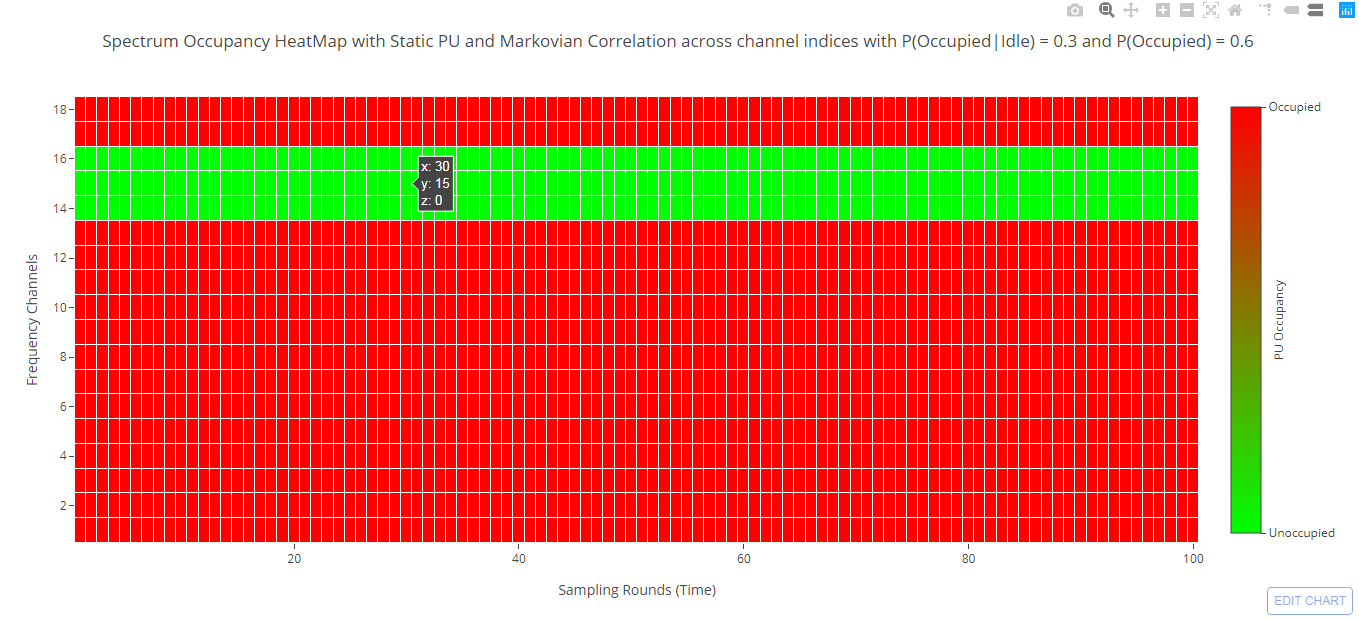
\includegraphics[width=1.0\textwidth]{Spectrum_Occupancy_Spatial_Markovian_Correlation.png}
\caption{Static PU Occupancy Behavior with Markovian Correlation across channel indices}
\label{fig:mesh1}
\centering
\end{figure}
\begin{figure}[t]
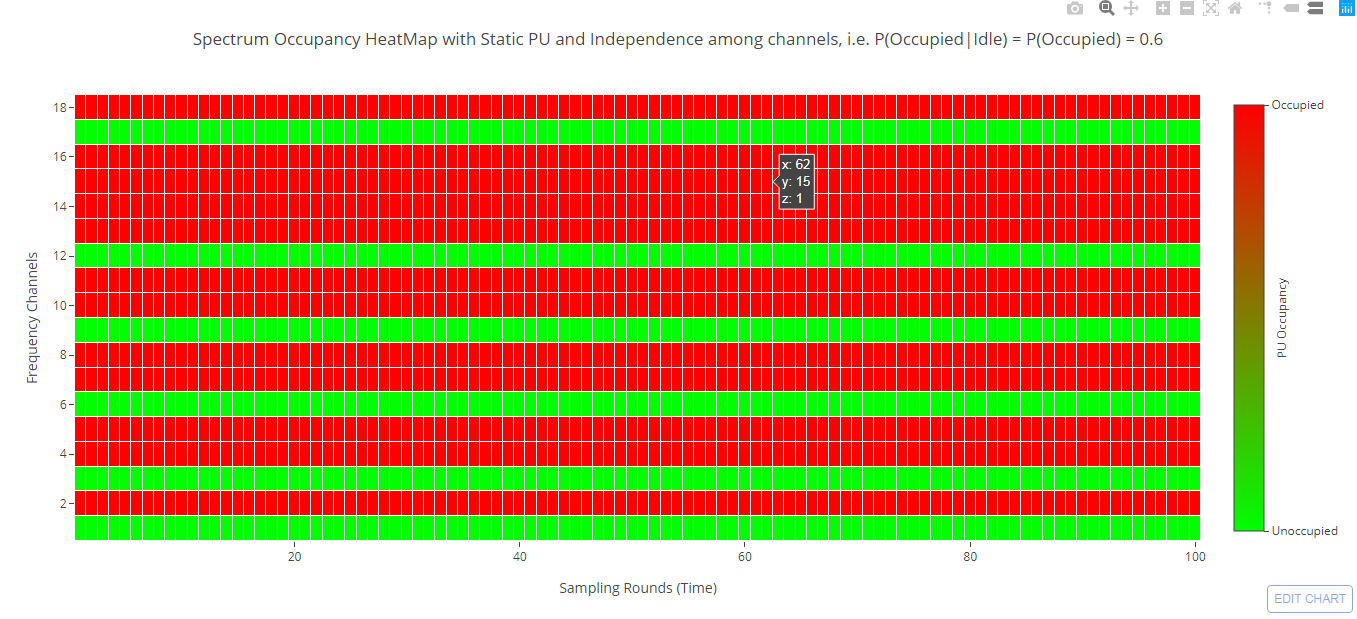
\includegraphics[width=1.0\textwidth]{Spectrum_Occupancy_Spatial_Independence_2.png}
\caption{Static PU Occupancy Behavior with independence among channels $\mathbb P(Occupied|Idle)\ =\ \mathbb P(Occupied)\ =\ 0.6$}
\label{fig:mesh2}
\centering
\end{figure}
\subsection{Visualization of Spatially Correlated PU Occupancy Behavior}
The following visualization results illustrate the Occupancy Behavior of the Primary User in a wideband spectrum of interest consisting of 18 frequency bands observed over 100 sampling rounds. The PU behavior is assumed to be static (constant across time).
\newline
\begin{itemize}
    \item Figure 1 depicts the PU Occupancy Behavior across time indices (sampling rounds) and across channel indices (frequency bands) assuming that a Markovian correlation exists across the channel indices based on the System Model detailed in the previous subsection. Specifically,
    \[\mathbb P(Occupied)\ =\ \mathbb P(X_i\ =\ 1)\ =\ \Pi\ =\ 0.6\]
    \[\mathbb P(Occupied|Idle)\ =\ \mathbb P(X_j = 1|X_i = 0)\ =\ p\ =\ 0.3\]
    \[\mathbb P(Idle|Occupied)\ =\ \mathbb P(X_j = 0|X_i = 1)\ =\ q\ =\ \frac{p(1-\Pi)}{\Pi}\ =\ 0.2\]
    \item Figure 2 depicts the PU Occupancy Behavior across time indices (sampling rounds) and across channel indices (frequency bands) assuming independence among channels, i.e,
    \[\mathbb P(Occupied|Idle)\ =\ \mathbb P(X_j = 1|X_i = 0)\ =\ p\ =\ \mathbb P(Occupied)\ =\ \mathbb P(X_i\ =\ 1)\ = \Pi\ =\ 0.6\]
\end{itemize}
\subsection{The Estimator}
\textbf{Given}: The observations of the K frequency sub-bands in the wideband spectrum of interest, i.e. $Y_1,\ Y_2,\ Y_3,\ .....,\ Y_K$
\\\textbf{Assuming} the state transition probability matrix $A$ and the array of initial probabilities $\Pi$ are known.
\\\textbf{From the observation model}, we already know that the emission probabilities are given by,
\[\mathbb P(Y_k|X_k = x_k)\ \sim \mathcal{CN}(0,\ \sigma_H^2x_k+\sigma_V^2)\]
Now, the problem of estimating a sequence of states across the frequency bands in a Hidden Markov Model can be solved using Dynamic Programming to give us the most likely sequence of hidden states called the \textbf{Viterbi Path} based on the sequence of noisy observations of the true states of the frequency sub-bands.
\\From the above statements we can write,
\begin{equation*}
    \mathbb P(\vec{X}=\vec{x}) = \mathbb P(X_1=x_1) \prod_{k=2}^{K} \mathbb P(X_k=x_k|X_{k-1}=x_{k-1})
\end{equation*}
Now, the optimization problem can be written as follows,
\begin{equation}\label{7}
    \vec{x}^* = argmax_{\vec{x}} \mathbb P(\vec{X}|\vec{Y})
\end{equation}
Here,
$\vec{Y}$ represents the observation vector consisting of the observations of the K sub-bands given by equation (\ref{2}), as shown below,
\[\vec{Y}\ =\ [{Y}_1,\ {Y}_2,\ ....,\ {Y}_K]^T\]
In other words,
\[\vec{x}^*\ represents\ the\ Viterbi\ path\ across\ frequency\ sub-bands\]
\[\vec{Y}\ represents\ the\ sequence\ of\ observations\ across\ frequency\ sub-bands\]
This argmax problem can be re-written as a maximization problem of the joint distribution due to the proportional relation between the joint and the conditional. Therefore, Equation (\ref{7}) can be written as,
\begin{equation}\label{8}
    V_{i}^{(j)}\ =\ max_{x_1,x_2,...,x_{i-1}}\mathbb P(y_1,y_2,...,y_{i-1},x_1,x_2,...,x_{i-1},y_i,x_{i}=j)
\end{equation}
Here, $V_{i}^{(j)}$ represents \textbf{a value function in our optimization problem tracking the sequence of states of sub-bands that maximize the joint distribution of states and observations as detailed in Equation (\ref{8})}.
\\Now, for the $(i+1)^{th}$ sub-band in state $l$, repeating the same step, we have,
\begin{equation}\label{9}
    V_{i+1}^{(l)}\ =\ max_{x_1,x_2,...,x_i}\mathbb P(y_1,y_2,...,y_i,x_1,x_2,...,x_i,y_{i+1},x_{i+1}=l)
\end{equation}
Using the definition of conditional probability, we have,
\begin{equation}\label{10}
    V_{i+1}^{(l)}\ =\ max_{x_1,x_2,...,x_i}\mathbb P(y_{i+1},x_{i+1}=l|y_1,y_2,...,y_i,x_1,x_2,...,x_i)\\\mathbb P(y_1,y_2,...,y_i,x_1,x_2,...,x_i)
\end{equation}
Now, from the Markov Property, we have,
\begin{equation}\label{11}
    V_{i+1}^{(l)}\ =\ max_{x_1,x_2,...,x_i}\mathbb P(y_{i+1},x_{i+1}=l|x_i)\mathbb P(y_1,y_2,...,y_i,x_1,x_2,...,x_i)
\end{equation}
Pushing the maximization operator in,
\begin{equation}\label{12}
    V_{i+1}^{(l)}\ =\ max_{j}[\mathbb P(y_{i+1},x_{i+1}=l|x_i=j)max_{x_1,x_2,...,x_{i-1}}[\mathbb P(y_1,y_2,...,y_{i-1},x_1,x_2,...,x_{i-1},y_i,x_i=j)]]
\end{equation}
Using Equation (\ref{8}),
\begin{equation}\label{13}
    V_{i+1}^{(l)}\ =\ max_{j}[\mathbb P(y_{i+1},x_{i+1}=l|x_i=j)V_i^{(j)}]
\end{equation}
We know that, for three random variables R, U, and W,
\[\mathbb P(R,U|W)\ =\ \mathbb P(U|R,W)\mathbb P(R|W)\]
Using this, we have,
\begin{equation}\label{14}
    V_{i+1}^{(l)}\ =\ max_{j}[\mathbb P(y_{i+1}|x_{i+1}=l,x_i=j)\mathbb P(x_{i+1}=l|x_i=j)V_i^{(j)}]
\end{equation}
\begin{equation}\label{15}
    V_{i+1}^{(l)}\ =\ max_{j}[\mathbb P(y_{i+1}|x_{i+1}=l)\mathbb P(x_{i+1}=l|x_i=j)V_i^{(j)}]
\end{equation}
Let, $m_l(y_{i+1})$ be the emission probability, i.e. the probability of emission of observation $y_{i+1}$ in state $l$.
\\Let, $a_{jl}$ be the state transition probability.
Then, 
\begin{equation}\label{16}
    V_{i+1}^{(l)}\ =\ m_l(y_{i+1})\ max_{j}[a_{jl}V_i^{(j)}]
\end{equation}
Here, from the observation model,
\[m_l(y_{i+1})\ \sim \mathcal{CN}(0,\ \sigma_H^2l+\sigma_V^2)\]
And, from the system's Markov model,
\[a_{jl}\ \in\ A,\ :\ a_{jl}\ =\ \mathbb P(x_{i+1}=l|x_i=j)\]
Equation (\ref{16}) constitutes the \textbf{Forward Recursion aspect of the Viterbi algorithm}.
\\Now, we analytically derive the \textbf{Backtrack feature of the Viterbi algorithm} below.
\\The state of the $K^{th}$ sub-band, i.e the last state in the Viterbi path is given by,
\begin{equation}\label{17}
    k^*\ =\ argmax_k\ V_K^{(k)}
\end{equation}
This can be written as follows,
\begin{equation}\label{18}
    k^*\ =\ argmax_k\ max_{x_1,x_2,...,x_{K-1}}\ \mathbb P(x_1,x_2,...,x_{K-1},x_K=k,y_1,y_2,...y_K)
\end{equation}
Essentially, the idea here is to prove the an earlier sub-band in the sequence is in a certain state given that a later sub-band in the sequence is in a certain state.
\\So,
\\\textbf{Given}: $x_{i+1}=l^*$ is the state of the $(i+1)^{th}$ sub-band in the most likely state sequence.
\\\textbf{To find an analytical solution} for the state of the $i^{th}$ sub-band in the most likely state-sequence.
\\Consider the pointer,
\[Ptr_{i+1}\ =\ argmax_j\ (a_{jl}V_{i}^{(j)})\]
Now, substituting in the definitions of the state transition probabilities and the value function,
\begin{equation}\label{19}
    Ptr_{i+1}=argmax_j\ \mathbb P(x_{i+1}=l^*|x_{i}=j)\ max_{x_1,x_2,...,x_{i-1}}\mathbb P(y_1,y_2,...,y_{i-1},x_1,x_2,...,x_{i-1},y_i,x_{i}=j)
\end{equation}
Moving the constant in or taking max operator outside,
\begin{equation}\label{20}
    Ptr_{i+1}=argmax_j\ max_{x_1,x_2,...,x_{i-1}}\ \mathbb P(x_{i+1}=l^*|x_{i}=j)\mathbb P(y_1,y_2,...,y_{i-1},x_1,x_2,...,x_{i-1},y_i,x_{i}=j)
\end{equation}
We can write Equation (\ref{20}) as,
\begin{equation}\label{21}
    \begin{aligned}
        Ptr_{i+1}=argmax_j\ max_{x_1,x_2,...,x_{i-1}}\ \mathbb P(x_{i+1}=l^*|x_1,x_2,...,x_{i-1},x_{i}=j,y_1,y_2,...,y_{i-1},y_{i})\\\mathbb P(y_1,y_2,...,y_{i-1},x_1,x_2,...,x_{i-1},y_i,x_{i}=j)
    \end{aligned}
\end{equation}
Using Chain Rule, this product becomes the joint distribution,
\begin{equation}\label{22}
        Ptr_{i+1}=argmax_j\ max_{x_1,x_2,...,x_{i-1}}\ \mathbb P(x_{i+1}=l^*,x_1,x_2,...,x_{i-1},x_{i}=j,y_1,y_2,...,y_{i-1},y_{i})
\end{equation}
Adding a constant to the argmax operation, i.e. $j$ should not feature in this constant, we have,
\begin{equation}\label{23}
    \begin{aligned}
        Ptr_{i+1}=argmax_j\ (max_{x_{i+1},x_{i+2},...,x_K}\ \mathbb P(x_{i+2},x_{i+3},...,x_K,y_{i+1},y_{i+2},...,y_{K}|x_{i+1}=l^*))\\max_{x_1,x_2,...,x_{i-1}}\ \mathbb P(x_{i+1}=l,x_1,x_2,...,x_{i-1},x_{i}=j,y_1,y_2,...,y_{i-1},y_{i}))
    \end{aligned}
\end{equation}
\begin{equation}\label{24}
    \begin{aligned}
        Ptr_{i+1}=argmax_j\ max_{x_{i+1},x_{i+2},...,x_K}\ max_{x_1,x_2,...,x_{i-1}}\ \mathbb P(x_{i+2},x_{i+3},...,x_K,y_{i+1},y_{i+2},...,y_{K}|x_{i+1}=l^*)\\\mathbb P(x_{i+1}=l,x_1,x_2,...,x_{i-1},x_{i}=j,y_1,y_2,...,y_{i-1},y_{i})
    \end{aligned}
\end{equation}
We can write Equation (\ref{24}) as follows due to the independence relation exhibited by the Markov Model,
\begin{equation}\label{25}
    \begin{aligned}
        Ptr_{i+1}=argmax_j\ max_{x_{i+1},x_{i+2},...,x_K}\ max_{x_1,x_2,...,x_{i-1}}\mathbb P(x_{i+2},x_{i+3},...,x_K,y_{i+1},y_{i+2},...,y_{K}|x_{i+1}=l^*,\\x_{i}=j,x_{i-1},...,x_1,y_{i},y_{i-1},...,y_1)\mathbb P(x_{i+1}=l,x_1,x_2,...,x_{i-1},x_{i}=j,y_1,y_2,...,y_{i-1},y_{i})
    \end{aligned}
\end{equation}
Using Chain Rule again and consolidating the max operator,
\begin{equation}\label{26}
    \begin{aligned}
        Ptr_{i+1}=argmax_j\ max_{x_1,x_2,...,x_{i-1},x_{i+1},x_{i+2},...,x_K}\ \mathbb P(x_{i+2},x_{i+3},...,x_K,x_{i+1}=l^*,x_{i}=j,x_{i-1},...,x_1,\\y_{i+1},y_{i+2},...,y_{K},y_{i},y_{i-1},...,y_1)
    \end{aligned}
\end{equation}
Now, the right-hand side of Equation (\ref{26}) corresponds to the state of the $i^{th}$ sub-band in most-likely state sequence.
\\Therefore,
\begin{equation}\label{27}
    \begin{aligned}
        Ptr_{i+1}\ =\ x_i*\ =\ j*
    \end{aligned}
\end{equation}
This constitutes an overlapping sub-problems solution which can be solved using Dynamic Programming. The idea is to recursively traverse through the Trellis diagram to find the next state which maximizes the probability of the traversed path. Using the analytical results obtained above, we can now write the algorithm.
\subsection{The Algorithm}
\begin{flushleft}
\textbf{Initialization}: Initial probabilities, $\mathbb{P}(X_k\ =\ 1)\ =\ \Pi$ and $\mathbb{P}(X_k\ =\ 0)\ =\ 1-\Pi$ are known.
\\\textbf{Forward Recursion}: $V_j^{(r)}\ =\ m_r(y_j)\ max_{l}[a_{lr}V_{j-1}^{(l)}]$
\\\textbf{Backtrack}: $Ptr_j\ =\ argmax_l\ (a_{lr}\ V_{j-1}^{(l)})$ and $x_{i-1}^*\ =\ Ptr_{i}$
\\\textbf{Termination}: $\mathbb P(\vec{y},\vec{x}^*)\ =\ max_k\ (V_K^{(k)})$
\end{flushleft}
\subsection{Simulation Results}
Let,
\[x_i\ =\ 1\ imply\ that\ frequency\ band\ i\ is\ Occupied\]
\[x_i\ =\ 0\ imply\ that\ frequency\ band\ i\ is\ Idle\]
The emission probabilities are obtained from the Gaussian Observation Model where,
\[Y_k(i) = H_kX_k(i) + V_k(i),\ and\]
\[m_l(y_{i+1})\ \sim \mathcal{CN}(0,\ \sigma_H^2l+\sigma_V^2)\]
Here,
\\$V_k(i)\ \sim\ \mathcal{CN}(0,\ \sigma_V^2)$ represents the circular-symmetric complex Gaussian noise sample
\\$H_k\ \sim\ \mathcal{CN}(0,\ \sigma_H^2)$ represents the $k^{th}$ DFT coefficient of the impulse response $h(n)$ of the channel in between the PU and the SU receiver
\\\textbf{The start probabilities $\Pi\ =\ \mathbb P(X_i\ =\ 1)$ are fixed at 0.60}.
If $p\ =\ \mathbb P(1|0)$ and $q\ =\ \mathbb P(0|1)$, then we can write the relation between $p$ and $q$ as follows,
\[\Pi\ =\ \frac{p}{p+q}\]
\textbf{Varying $p$ from $0.030\ to\ \Pi$}, where if $p\ =\ \Pi$ corresponds to independence among bands because $\mathbb P(1|0)\ =\ \mathbb P(1)$ and $\mathbb P(0|1)\ =\ \mathbb P(0)$, we get a plot of $Detection\ Accuracy\ v/s\ p$ as depicted in Figure 3. Multiple independent trials have been run to smooth the curve.
\begin{figure}[t]
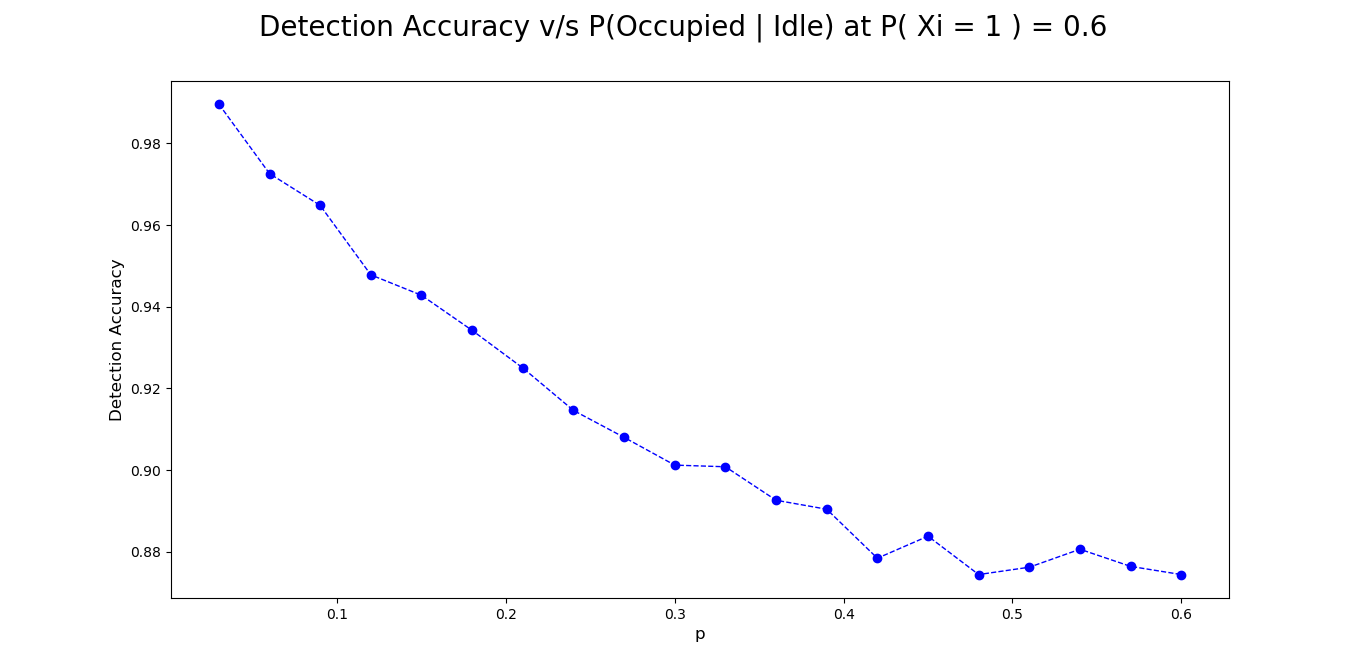
\includegraphics[width=1.0\textwidth]{DetectionAccuracy_v_p_test_3_final.png}
\caption{Detection Accuracy v/s p for $1000$ observations per band averaged over 50 independent trials with $\Pi\ =\ 0.60$ and $p$ varied from $0.03$ to $\Pi$. This plot corresponds to a linear noisy observation model with the system modelled as an HMM. The true states for the 18 frequency bands are generated using a custom Markov state generator $\forall p\ and\ \forall q$ with a fixed $\Pi\ =\ 0.6$.}
\label{fig:mesh3}
\centering
\end{figure}
\clearpage
\section{Static PU with Channel Correlation and Incomplete Information}
\subsection{Observation Model}
\begin{equation}\label{28}
    Y_k(i) = H_kX_k(i) + V_k(i)
\end{equation}
where,
\\$i\ \in\ \{1,\ 2,\ 3,\ .........,\ T\}$ represents the index of the observation
\\\textbf{NOTE}: Multiple observations of all the frequency bands are made by the SU for training the algorithm and averaging the results over numerous iterations. However, the PU occupancy behavior in this case remains static over time.
\\$k\ \in\ \{1,\ 2,\ 3,\ .........,\ K\}$ represents the index of the sub-band
\\$V_k(i)\ \sim\ \mathcal{CN}(0,\ \sigma_V^2)$ represents the zero-mean additive Gaussian noise sample
\\$H_k\ \sim\ \mathcal{CN}(0,\ \sigma_H^2)$ represents the $k^{th}$ DFT coefficient of the impulse response $h(n)$ of the channel in between the PU and the SU receiver
\\The PU occupancy behavior in each sub-band $b_k\ \in\ B$ is modelled as $X_k$ taking two possible values $0\ and\ 1$. Therefore, the PU occupancy behavior in the entire wideband spectrum of interest discretized into narrow-band frequency components can be modelled as a vector of size $|B|\ =\ K$ such that,
\begin{equation}\label{29}
    \vec{X} = [X_1, X_2, X_3, ........., X_K]^T \in \{0,1\}^K
\end{equation}
\subsection{System Model}
The true states encapsulate the actual behavior of the PU which is an unobserved Markov process and the measurements at the SU are noisy observations of the true states which are modelled to be the observed states of a Hidden Markov Model.
For some sub-band $j\ \in\ \{2,\ 3,\ 4,\ .....,\ K\}$, the system is assumed to satisfy the Markov property as shown below,
\[\mathbb P(X_{j}(i)|X_{j-1}(i),\ X_{j-2}(i),\ .....,\ X_1(i))\ =\ \mathbb P(X_{j}(i)|X_{j-1}(i)),\ for\ j>1,\]
\[And,\ we\ will\ use\ \mathbb P(X_1(i))\ for\ j=1.\]
Since \textbf{the PU is assumed to be static in the period of our estimation}, we can write the above assumption as,
\[\mathbb P(X_{j}|X_{j-1},\ X_{j-2},\ .....,\ X_1)\ =\ \mathbb P(X_{j}|X_{j-1}),\ for\ j>1,\]
\[And,\ we\ will\ use\ \mathbb P(X_1)\ for\ j=1.\]
Now, we know that,
\[\vec{X}\ =\ [X_1,\ X_2,\ X_3,\ ......,\ X_K]^T\] which realizes as,
\[\vec{x}\ =\ [x_1,\ x_2,\ x_3,\ ......,\ x_K]^T\]
So,
\begin{equation}\label{30}
    \mathbb P(\vec{X}=\vec{x}) = \mathbb P(X_1=x_1) \prod_{k=2}^{K} \mathbb P(X_k=x_k|X_{k-1}=x_{k-1})
\end{equation}
Moreover, we also assume that the Markov Property is satisfied when we traverse the spectrum in the descending order of the channel indices, i.e, the reverse direction. Mathematically,
\begin{equation*}
\mathbb P(\vec{X}=\vec{x})=\mathbb P(X_K=x_K)\prod_{k=1}^{K-1} \mathbb P(X_{k}=x_k|X_{k+1}=x_{k+1})
\end{equation*}
\textbf{Assuming there is a single PU and a single SU making observations}, we have, from the observation model,
\begin{equation}\label{31}
    \mathbb P(Y_k|X_k = x_k)\ \sim \mathcal{CN}(0,\ \sigma_H^2x_k+\sigma_V^2)
\end{equation}
In this extension, the SU does not sense all $|B|\ =\ K$ frequency bands in the wideband spectrum of interest. Instead, a subset $M\ <\ K$ frequency bands are sensed based on recommendations given a Bandit or a Reinforcement Learning agent. Let the set of these "incomplete" observations be given as,
\[\vec{Y}\ =\ [y_1,\ y_2,\ \phi,\ ...,\ \phi,....,\ y_m,\ \phi,\ ...,\ y_K]^T\]
where, $\vec{Y}$ represents the observation vector with $\phi$ filled in for frequency bands which have not been observed.
Based on this System Model and Observation Model, the state sequence estimation procedure detailed in Section 1 (\textit{Static PU with complete observations}) can be modified to account for missing observations as described in Section 2.3.
\subsection{The Estimator}
Assuming a static PU across time, a linear, noisy observation model, and a Markovian correlation across the frequency channels, the optimization problem can be stated as follows.
\begin{equation}\label{32}
    \vec{x}^* = argmax_{\vec{x}} \mathbb P(\vec{X}|\vec{Y})
\end{equation}
\[\vec{x}^* = argmax_{\vec{x}} \mathbb P(\vec{X}\ =\ [x_1,\ x_2,\ x_3,\ ......,\ x_K]^T\ |\ \vec{Y}\ =\ [y_1,\ y_2,\ \phi,\ ...,\ \phi,....,\ y_m,\ \phi,\ ...,\ y_K]^T)\]
For $X_1 = x_1$, i.e. \textbf{Initialization},
\[V_1^{(r)}\ =\ m_r(y_1)\pi_r,\ if\ y_1\ \neq\ \phi\]
\[V_1^{(r)}\ =\ \pi_r,\ if\ y_1\ = \phi\]
where,
\[m_r(y_1)\ \sim \mathcal{CN}(0,\ \sigma_H^2r+\sigma_V^2),\]
\[\pi_r\ =\ \mathbb{P}(X_1\ =\ r)\]
\[r\ \in\ \{0,\ 1\}\]
Now, moving on to the \textbf{Forward Recursion aspect},
\[V_j^{(r)}\ =\ m_r(y_j)\ max_l[a_{lr}V_{j-1}^{(l)}],\ if\ y_j\ \neq\ \phi\]
\[V_j^{(r)}\ =\ max_l[a_{lr}V_{j-1}^{(l)}],\ if\ y_j\ =\ \phi\]
where,
\[m_r(y_j)\ \sim \mathcal{CN}(0,\ \sigma_H^2r+\sigma_V^2),\]
\[j\ \in\ \{2,\ 3,\ 4,\ ......,\ K\}\]
\[l,\ r\ \in\ \{0,1\}\]
Now, moving on to the \textbf{Backtracking aspect},
\[Ptr_j\ =\ argmax_l(a_{lr}V_{j-1}^{(l)})\]
\[k^*\ =\ argmax_k(V_K^{(k)})\]
\[x_{i-1}^*\ =\ Ptr_i\]
There are other approaches to this "missing observations" problem of state estimation. For example, approaches like Gluing and Multi-sequences are discussed in Ref [\ref{10}]. Similar models are used in Automatic Speech Recognition with Missing Data (ASR with MD) as detailed in Ref [\ref{11}].
\subsection{Simulation Results}
The following results illustrate the PU Occupancy Behavior Estimation Algorithm with Markovian Correlation across channel indices and with incomplete information, i.e. missing observations. The channel selection strategy is simulated in two ways: Uniform Sampling and Random Sampling. In the Uniform Sampling/Uniform Sensing strategy, the step size between consecutive channels is incremented by 1 in each cycle while in the Random Sampling/Random Sensing strategy, a random number of channels are sensed from the discretized wideband spectrum of interest.
\\The simulation model consists of 18 channels with 100 samples per channel over 50 iteration cycles.
\\$\mathbb P(Occupied|Idle)\ =\ p$ is incremented in steps of $0.03$ from $0.03$ all the way up to $\mathbb P(Occupied)\ =\ \Pi\ =\ 0.6$ and for a given value of $p$, the detection accuracy is calculated and averaged out over multiple iteration cycles.
\\The detection accuracy is then plotted against $\mathbb P(Occupied|Idle)\ =\ p$.
\begin{itemize}
    \item In this run, only the even channels in the discretized wideband spectrum of interest are sensed, i.e. the channel selection strategy is \{0, 2, 4, 6, 8, 10, 12, 14, 16\}. The Detection Accuracy v/s $\mathbb P(Occupied|Idle)$ plot is depicted in Figure 4. The blue curve corresponds to the detection accuracy of the sensed channels which, as expected, should fare better compared to the detection accuracy of the un-sensed channels (the red curve).
    \item Figure 5 depicts the plot of Detection Accuracy versus $\mathbb P(Occupied|Idle)$ for a Uniform Sensing Channel Selection Strategy
    \item Figure 6 depicts the plot of Detection Accuracy versus $\mathbb P(Occupied|Idle)$ for a Uniform Sensing Channel Selection Strategy with the 'Duals' of the channels sensed in Figure 5, i.e. the channels that were missed in runs of Figure 5 are sensed here to get an understanding on the "regret" of the channel selection strategy.
    \item Figure 7 depicts the plot of Detection Accuracy versus $\mathbb P(Occupied|Idle)$ for a Random Sensing Channel Selection Strategy
    \item Figure 8 depicts the plot of Detection Accuracy versus $\mathbb P(Occupied|Idle)$ for a Random Sensing Channel Selection Strategy with the 'Duals' of the channels sensed in Figure 7, i.e. the channels that were missed in runs of Figure 7 are sensed here to get an understanding on the "regret" of the channel selection strategy.
\end{itemize}
\begin{figure}[t]
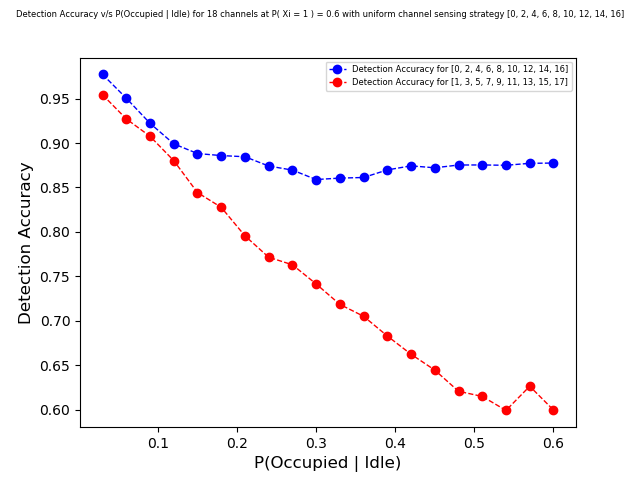
\includegraphics[width=1.0\textwidth]{Uniform_Channel_Sensing_1.png}
\caption{Detection Accuracy v/s $\mathbb P(Occupied\ |\ Idle)$ for 18 channels with Markovian Correlation across channel indices and missing observations where the channel selection strategies are recommended by a Uniform Sampling process. Here, the plot presents a comparison of the detection accuracy performances between the sensed channels and the un-sensed channels when only the even channels in the discretized wideband spectrum of interest have been sensed by the SU.}
\label{fig:mesh4}
\centering
\end{figure}
\begin{figure}[t]
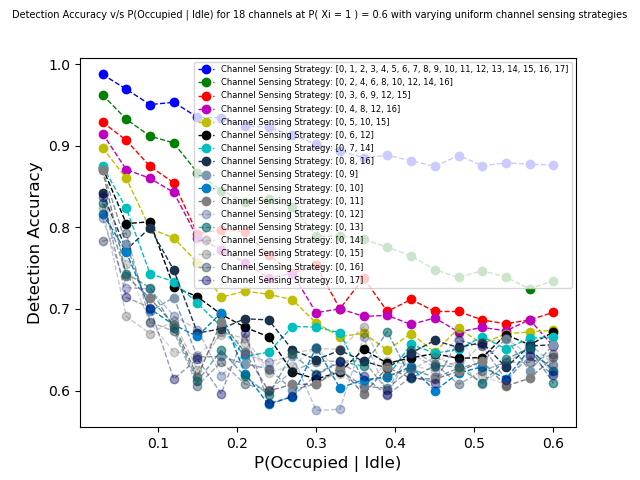
\includegraphics[width=1.0\textwidth]{Uniform_Channel_Sensing.png}
\caption{Detection Accuracy v/s $\mathbb P(Occupied\ |\ Idle)$ for 18 channels with Markovian Correlation across channel indices and missing observations where the channel selection strategies are recommended by a Uniform Sampling process.}
\label{fig:mesh5}
\centering
\end{figure}
\begin{figure}[t]
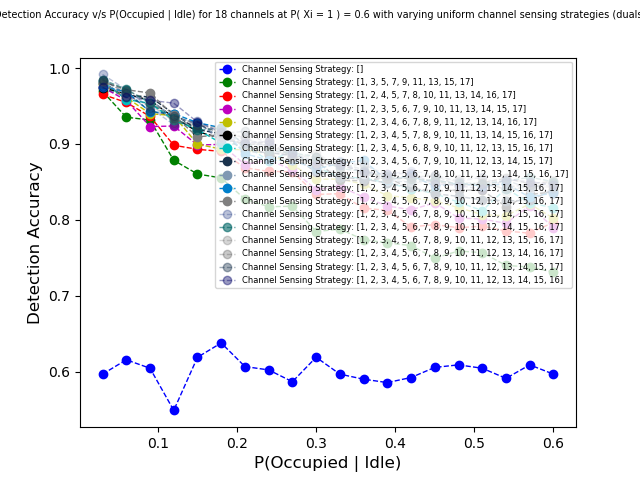
\includegraphics[width=1.0\textwidth]{Uniform_Channel_Sensing_Duals.png}
\caption{Detection Accuracy v/s $\mathbb P(Occupied\ |\ Idle)$ for 18 channels with Markovian Correlation across channel indices and missing observations where the channel selection strategies involve the Duals of the channels employed in Figure 5.}
\label{fig:mesh6}
\centering
\end{figure}
\begin{figure}[t]
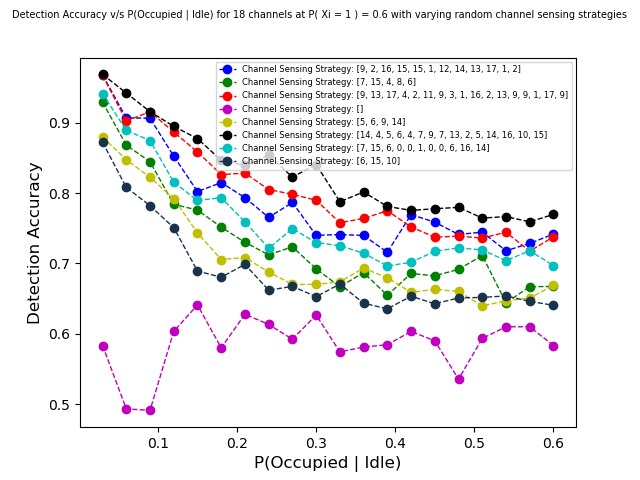
\includegraphics[width=1.0\textwidth]{Random_Channel_Sensing.png}
\caption{Detection Accuracy v/s $\mathbb P(Occupied\ |\ Idle)$ for 18 channels with Markovian Correlation across channel indices and missing observations where the channel selection strategies are recommended by a Random Sampling process.}
\label{fig:mesh7}
\centering
\end{figure}
\begin{figure}[t]
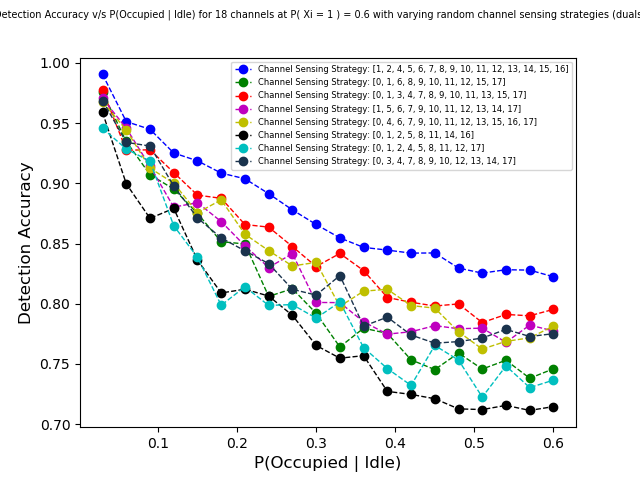
\includegraphics[width=1.0\textwidth]{Random_Channel_Sensing_Duals.png}
\caption{Detection Accuracy v/s $\mathbb P(Occupied\ |\ Idle)$ for 18 channels with Markovian Correlation across channel indices and missing observations where the channel selection strategies involve the Duals of the channels employed in Figure 7.}
\label{fig:mesh8}
\centering
\end{figure}
\clearpage
\section{Dynamic PU with Temporal Correlation and Channel Correlation with Complete Information}
\subsection{Observation Model}
Persisting the same observation model as in the previous sections,
\begin{equation}\label{33}
    Y_k(i) = H_kX_k(i) + V_k(i)
\end{equation}
where,
\\$i\ \in\ \{1,\ 2,\ 3,\ .........,\ T\}$ represents the index of the observation
\\$k\ \in\ \{1,\ 2,\ 3,\ .........,\ K\}$ represents the index of the sub-band
\\$V_k(i)\ \sim\ \mathcal{CN}(0,\ \sigma_V^2)$ represents the zero-mean additive Gaussian noise sample
\\$H_k\ \sim\ \mathcal{CN}(0,\ \sigma_H^2)$ represents the $k^{th}$ DFT coefficient of the impulse response $h(n)$ of the channel in between the PU and the SU receiver
\\The PU occupancy behavior in each sub-band $b_k\ \in\ B$ is modelled as $X_k$ taking two possible values $0\ and\ 1$. Therefore, the PU occupancy behavior in the entire wideband spectrum of interest discretized into narrow-band frequency components can be modelled as a vector of size $|B|\ =\ K$ such that,
\begin{equation}\label{34}
    \vec{X} = [X_1, X_2, X_3, ........., X_K]^T \in \{0,1\}^K
\end{equation}
Solving for the mean and variance of $Y_k(i)$ from (\ref{33}) with $X_k(i)\ =\ x_k$, we get,
\begin{equation}\label{35}
    \mathbb E[Y_k(i) | X_k(i) = x_k] = 0
\end{equation}
\begin{equation}\label{36}
    Var[Y_k(i) | X_k(i) = x_k] = \sigma_H^2x_k + \sigma_V^2
\end{equation}
Therefore,
\[Y_k(i)\ \sim\ \mathcal{CN}(0,\ \sigma_H^2x_k + \sigma_V^2)\]
\subsection{System Model}
The system model comprises a \textbf{2D Markov Chain: one across time and one across frequency bands - all the frequency bands in the wideband spectrum of interest are sensed by the SU in each sampling round $t$}. We'll see the next extension of this work (PU Occupancy Behavior Estimation with Time and Channel Markovian Correlation and Incomplete Information) in Section 4 of this document.
\\The \textbf{transition probabilities matrix} for PU Occupancy Behavior transitions, i.e $0\longrightarrow1$ or $1\longrightarrow0$ across both time and frequency is given by,
\[A\ is\ a\ matrix\ of\ elements\ a_{mnr}\ =\ [A]_{mnr}\ such\ that\ a_{mnr}\ =\ \mathbb P(x_{tk}\ =\ r\ |\ x_{t-1,k}\ =\ m,\ x_{t,k-1}\ =\ n)\]
where,
\[r,\ m,\ n\ \in\ \{0,1\}\ represents\ the\ PU\ occupancy\ state\ in\ a\ particular\ channel\ at\ a\ particular\ time\]
\[t\ \in\ \{2,\ 3,\ 4,\ .....,\ T\}\ represents\ the\ temporal\ index\]
\[k\ \in\ \{2,\ 3,\ 4,\ .....,\ K\}\ represents\ the\ channel\ index\]
From the observation model, the \textbf{emission probabilities} are given by,
\[m_r(y_{tk})\ =\ \mathbb P(y_{tk}\ |\ x_{tk}\ =\ r)\ \sim\ \mathcal{CN}(0,\ \sigma_H^2r+\sigma_V^2)\]
where,
\[r\ \in\ \{0,1\}\]
The \textbf{initial or start probabilities} are given as follows.
\[\Pi\ =\ \{\pi_r:\ \pi_r\ =\ \mathbb P(x_{tk}\ =\ r)\ for\ t\ =\ 1\ or\ k\ =\ 1,\ \forall\ r\ \in\ \{0,1\}\}\]
\subsection{Visualization of Temporally and Spatially Correlated PU behavior}
The following visualization results illustrate the Occupancy Behavior of the Primary User in a wideband spectrum of interest consisting of 18 frequency bands observed over 100 sampling rounds. The PU behavior is dynamic (varying across time).
\begin{itemize}
    \item Figure 9 depicts the PU Occupancy Behavior across time indices (sampling rounds) and across channel indices (frequency bands) assuming that a dual Markov chain exists- one across channels and one across sampling rounds. Mathematical details about the System Model are outlined in the previous subsection. Specifically, for both the Markov chains, 
    \[\mathbb P(Occupied|Idle)\ =\ \mathbb P(X_j = 1|X_i = 0)\ =\ p\ =\ 0.3\]
    \[\mathbb P(Occupied)\ =\ \mathbb P(X_i\ =\ 1)\ =\ \Pi\ =\ 0.6\]
    \item Figure 10 depicts the PU Occupancy Behavior across time indices (sampling rounds) and across channel indices (frequency bands) assuming independence among channels and among sampling rounds, i.e,
    \[\mathbb P(Occupied|Idle)\ =\ \mathbb P(X_j = 1|X_i = 0)\ =\ p\ =\ \mathbb P(Occupied)\ =\ \mathbb P(X_i\ =\ 1)\ = \Pi\ =\ 0.6\]
\end{itemize}
\begin{figure}[t]
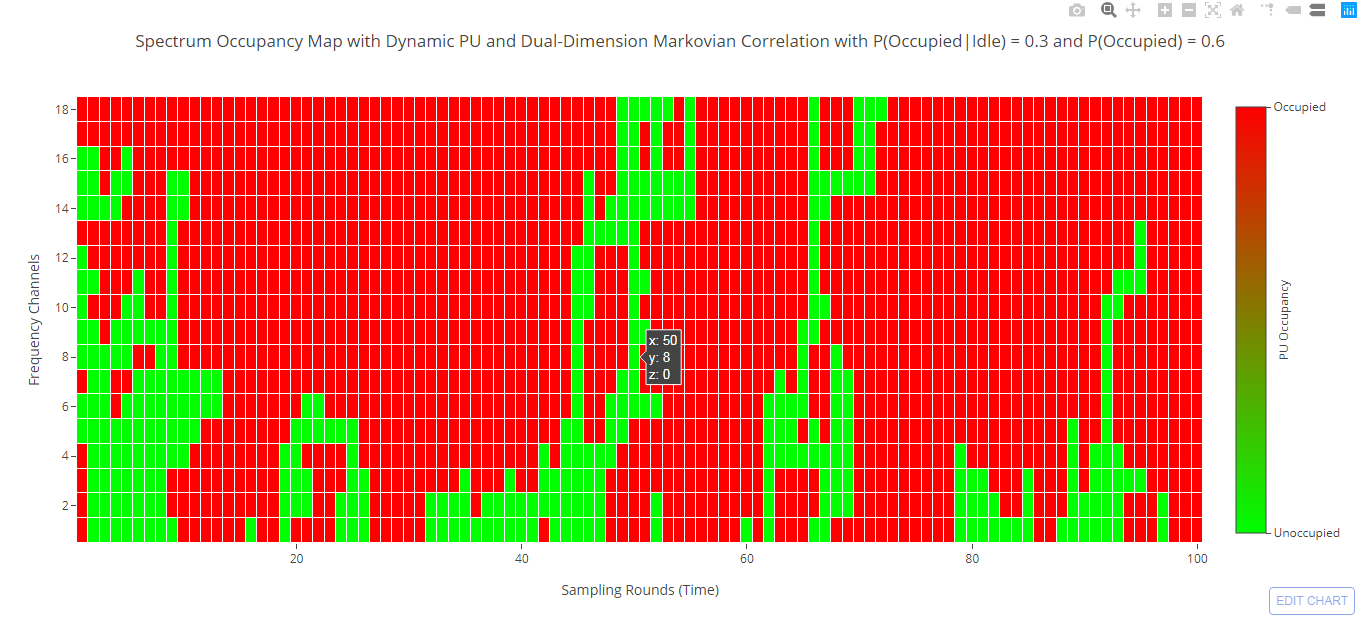
\includegraphics[width=1.0\textwidth]{Spectrum_Occupancy_SpatioTemporal_Markovian_Correlation.png}
\caption{Dynamic PU Occupancy Behavior with Markovian Correlation across channel indices and across time indices}
\label{fig:mesh9}
\centering
\end{figure}
\begin{figure}[t]
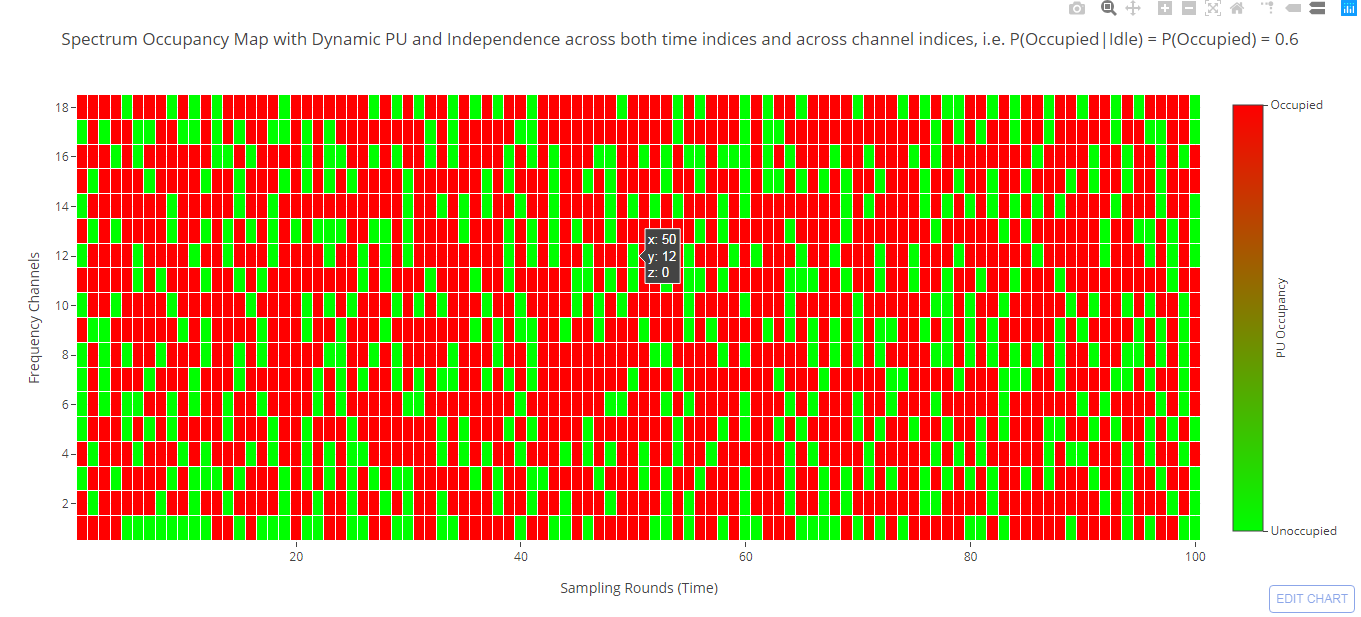
\includegraphics[width=1.0\textwidth]{Spectrum_Occupancy_SpatioTemporal_Independence_2.png}
\caption{Dynamic PU Occupancy Behavior with independence among channels and among sampling rounds}
\label{fig:mesh10}
\centering
\end{figure}
\subsection{The Estimator}
\subsubsection{Notations}
Let us first define the notations employed in this analytical derivation.
\\The set of all past observations required for the estimation of PU Occupancy in channel $k$ in sampling round $t$ is given as follows.
\[y_{1:t-1,1:k-1}\ =\ \{y_{t,1},y_{t,2},...,y_{t,k-1},y_{1,k},y_{2,k},...,y_{t-1,k}\}\]
\\The set of all past states required for the estimation of PU Occupancy in channel $k$ in sampling round $t$ is given as follows.
\[x_{1:t-1,1:k-1}\ =\ \{x_{t,1},x_{t,2},...,x_{t,k-1},x_{1,k},x_{2,k},...,x_{t-1,k}\}\]
\\The joint probability term while analyzing state-observation pair of channel $k$ which is in state $r \in \{0,1\}$ in sampling round $t$ is denoted as follows.
\[\mathbb P(y_{tk}, x_{tk}=r, y_{1:t-1,1:k-1}, x_{1:t-1,1:k-1})\]
The probability terms are simplified and the estimation algorithm's analytical expressions are derived in the upcoming subsubsections.
\subsubsection{Defining the Probability terms}
The joint probability term for analyzing the state-observation pair of channel $k$ which is in state $r \in \{0,1\}$ in sampling round $t$ is defined as follows. Note that, channel $k$ is in state $m \in \{0,1\}$ in sampling round $t-1$ and channel $k-1$ is in state $n \in \{0,1\}$ in sampling round $t$. Based on our System Model described subsection B of section III, the PU Occupancy state at location $(t,k)$ depends only on the PU Occupancy states at locations $(t-1,k)$ and $(t,k-1)$ respectively, i.e. the previous states both temporally and spatially.
\begin{equation*}
    \mathbb P(y_{tk}, x_{tk}=r, y_{1:t-1,1:k-1}, x_{1:t-1,1:k-1})
\end{equation*}
Using the definition of conditional probability, the joint probability term from above can be written as,
\begin{equation*}
    \mathbb P(y_{tk}, x_{tk}=r|y_{1:t-1,1:k-1}, x_{1:t-1,1:k-1})\mathbb P(y_{1:t-1,1:k-1}, x_{1:t-1,1:k-1})
\end{equation*}
Using the Markov property across both time indices (sampling rounds or iterations) and channel indices, the joint probability term from above can be written as,
\begin{equation*}
    \mathbb P(y_{tk}, x_{tk}=r|x_{t-1,k}=m,x_{t,k-1}=n)\mathbb P(y_{1:t-1,1:k-1}, x_{1:t-1,1:k-1})
\end{equation*}
Simplifying the conditional even further, the aforementioned joint probability term can be written as,
\begin{equation*}
        \mathbb P(y_{tk}|x_{tk}=r,x_{t-1,k}=m,x_{t,k-1}=n)\mathbb P(x_{tk}=r|x_{t-1,k}=m,x_{t,k-1}=n)\mathbb P(y_{1:t-1,1:k-1}, x_{1:t-1,1:k-1})
\end{equation*}
Since the observations depend only on the current state, the joint probability term can be further simplified as,
\begin{equation*}
        \mathbb P(y_{tk}|x_{tk}=r)\mathbb P(x_{tk}=r|x_{t-1,k}=m,x_{t,k-1}=n)\mathbb P(y_{1:t-1,1:k-1}, x_{1:t-1,1:k-1})
\end{equation*}
Using the definitions of emission and state transition probabilities from the System Model, the aforementioned joint probability term can be written as,
\begin{equation*}
        m_r(y_{tk})a_{mnr}\mathbb P(y_{1:t-1,1:k-1}, x_{1:t-1,1:k-1})
\end{equation*}
\subsubsection{Maximization of the Probabilities to arrive at the Forward and Backward Variables}
For the state estimation analysis, let's derive the analytical equations for a state element $x_{tk}\ =\ r$ and for the corresponding observation element $y_{tk}$. We'll now derive the forward and backward variables based on this \textit{node} and it's neighbors.
Let us first define the value function $V_{t-1,k-1}^{(l)}$ as follows.
\begin{equation}\label{37}
        V_{t-1,k-1}^{(l)}\ =\ max_{1:t-2,1:k-2}[\mathbb P(y_{1:t-2,1:k-2},x_{1:t-2,1:k-2},y_{t-1,k-1},x_{t-1,k-1}=l)]
\end{equation}
Here, $V_{t-1,k-1}^{(l)}$ represents the maximum probability of emission of $y_{t-1,k-1}$ with $x_{t-1,k-1}\ =\ l\ \in\ \{0,1\}$.
\\Now, since we have two dimensions (time indices and channel indices) in our System Model, we will have two flavors of value functions as discussed below. Let's first define $V_{t-1,k}^{(m)}$, i.e. the \textbf{horizontal transition across channel indices} with respect to $ V_{t-1,k-1}^{(l)}$ in the same way as in equation (\ref{37}).
\begin{equation}\label{38}
   V_{t-1,k}^{(m)}\ =\ max_{1:t-2,1:k-1}[\mathbb P(y_{1:t-2,1:k-1},x_{1:t-2,1:k-1},y_{t-1,k},x_{t-1,k}=m)]
\end{equation}
Similarly, let's define the value functions for time index traversal as follows.
Writing $V_{t,k-1}^{(n)}$, i.e. the \textbf{vertical transition across time indices} with respect to $ V_{t-1,k-1}^{(l)}$ in the same way as in equation (\ref{37}),
\begin{equation}\label{39}
    \begin{aligned}
        V_{t,k-1}^{(n)}\ =\ max_{1:t-1,1:k-2}[\mathbb P(y_{1:t-1,1:k-2},x_{1:t-1,1:k-2},y_{t,k-1},x_{t,k-1}=n)]
    \end{aligned}
\end{equation}
Now, let's define the \textbf{Forward Recursion} Value function for $V_{tk}^{(r)}$ using the analytical equations defined above.
From equation (\ref{37}),
\begin{equation}\label{40}
         V_{t,k}^{(r)}\ =\ max_{1:t-1,1:k-1}[\mathbb P(y_{1:t-1,1:k-1}, x_{1:t-1,1:k-1},y_{tk},x_{tk}=r)]
\end{equation}
Now, using the definition of conditional probability, we have,
\begin{equation}\label{41}
    V_{t,k}^{(r)}\ =\ max_{1:t-1,1:k-1}[\mathbb P(y_{tk}, x_{tk}=r|y_{1:t-1,1:k-1}, x_{1:t-1,1:k-1})\mathbb P(y_{1:t-1,1:k-1}, x_{1:t-1,1:k-1})]
\end{equation}
Since, we have a Markovian correlation across both time and frequency, we can apply the Markov property to equation (\ref{41}), to get,
\begin{equation}\label{42}
         V_{t,k}^{(r)}\ =\ max_{1:t-1,1:k-1}[\mathbb P(y_{tk}, x_{tk}=r|x_{t-1,k}=m,x_{t,k-1}=n)\mathbb P(y_{1:t-1,1:k-1}, x_{1:t-1,1:k-1})]
\end{equation}
Simplifying the conditional even further, we have,
\begin{equation}\label{43}
\begin{aligned}
    V_{t,k}^{(r)}\ =\ max_{1:t-1,1:k-1}[\mathbb P(y_{tk}|x_{tk}=r,x_{t-1,k}=m,x_{t,k-1}=n)\mathbb P(x_{tk}=r|x_{t-1,k}=m,x_{t,k-1}=n)\\\mathbb P(y_{1:t-1,1:k-1}, x_{1:t-1,1:k-1})]
\end{aligned}
\end{equation}
Since the observation in location $(t,k)$ depends only on the PU Occupancy state $x_{t,k}\ =\ r \in \{0,1\}$,
\begin{equation}\label{44}
    V_{t,k}^{(r)}\ =\ max_{1:t-1,1:k-1}[\mathbb P(y_{tk}|x_{tk}=r)\mathbb P(x_{tk}=r|x_{t-1,k}=m,x_{t,k-1}=n)\mathbb P(y_{1:t-1,1:k-1}, x_{1:t-1,1:k-1})]
\end{equation}
From the system model definitions of emission and transition probabilities, equation (\ref{44}) can be written as,
\begin{equation}\label{45}
    V_{t,k}^{(r)}\ =\ m_r(y_{tk})\ max_{1:t-1,1:k-1}[a_{mnr}\mathbb P(y_{1:t-1,1:k-1}, x_{1:t-1,1:k-1})]
\end{equation}
Factorizing the joint distribution into its independent constituent marginals and splitting the maximization operator, we have,
\begin{equation}\label{46}
    \begin{aligned}
         V_{t,k}^{(r)}\ =\ m_r(y_{tk})\ max_{(t,k-1),(t-1,k)}[a_{mnr}\  max_{1:k-1}[\mathbb P(y_{1:k-2},x_{1:k-1})]max_{1:t-1}[\mathbb P(y_{1:t-1},x_{1,t-1})]]
    \end{aligned}
\end{equation}
Using redundancy, equation (\ref{46}) can be written as,
\begin{equation}\label{47}
    \begin{aligned}
         V_{t,k}^{(r)}\ =\ m_r(y_{tk})\ max_{m,n}[a_{mnr}max_{1:k-2,1:t-1}[\mathbb P(y_{1:k-2},y_{t,k-1},y_{1:t-1},x_{1:k-2},x_{t,k-1}=n,x_{1:t-1})]\\max_{1:t-2,1:k-1}[\mathbb P(y_{1:t-2},y_{t-1,k},y_{1:k-1},x_{1:t-2},x_{t-1,k}=m,x_{1:k-1})]]]
    \end{aligned}
\end{equation}
Consolidating terms inside the joint probabilities, we have,
\begin{equation}\label{48}
    \begin{aligned}
         V_{t,k}^{(r)}\ =\ m_r(y_{tk})\ max_{m,n}[a_{mnr}max_{1:k-2,1:t-1}[\mathbb P(y_{1:k-2,1:t-1},y_{t,k-1},x_{1:k-2,1:t-1},x_{t,k-1}=n)]\\max_{1:t-2,1:k-1}[\mathbb P(y_{1:t-2,1:k-1},y_{t-1,k},x_{1:t-2,1:k-1},x_{t-1,k}=m)]]]
    \end{aligned}
\end{equation}
Now, we know from equations (\ref{38}) and (\ref{39}) that,
\begin{equation*}
   V_{t-1,k}^{(m)}\ =\ max_{1:t-2,1:k-1}[\mathbb P(y_{1:t-2,1:k-1},x_{1:t-2,1:k-1},y_{t-1,k},x_{t-1,k}=m)]
\end{equation*}
\begin{equation*}
    V_{t,k-1}^{(n)}\ =\ max_{1:t-1,1:k-2}[\mathbb P(y_{1:t-1,1:k-2},x_{1:t-1,1:k-2},y_{t,k-1},x_{t,k-1}=n)]
\end{equation*}
Using these results in equation (\ref{48}), we get,
\begin{equation}\label{49}
    \begin{aligned}
         V_{t,k}^{(r)}\ =\ m_r(y_{tk})max_{m,n}[a_{mnr}V_{t,k-1}^{(n)}V_{t-1,k}^{(m)}]
    \end{aligned}
\end{equation}
So, intuitively, the maximum probability of emission of $y_{tk}$ with the actual state of channel $k$ in sampling round $t$ depends on the previous element along the column vector (i.e. time) and the previous element along the row vector (i.e. channel) in addition to the probability of transitioning from $n \longrightarrow r$ horizontally and the probability of transitioning from $m \longrightarrow r$ vertically. The previous elements $(t,k-1)$ and $(t-1,k)$ depend on $V_{t-1,k-1}^{(l)}$.
\\Now, similar to the \textbf{backtracking procedure} in the 1D Viterbi algorithm, the Trellis diagram is traversed backwards from the final state to recover its two previous neighbors: one along the channel index and the other along the temporal index. This is done recursively until the entire Trellis has been traversed all the way back to the first state in the most probable state sequence (Viterbi path).
\\Mathematically,
\begin{equation}\label{50}
    \begin{aligned}
         x_{t-1,k-1}^*\ =\ l^*\ =\ argmax_{l}\{a_{mnr}\ V_{t,k-1}^{(n)}V_{t-1,k}^{(m)}\}
    \end{aligned}
\end{equation}
Using the analytical equations derived for both the \textbf{Forward Recursion phase and the Backtracking phase of our 2D Viterbi algorithm}, the final algorithm is given as follows.
\subsection{The Algorithm}
\begin{flushleft}
\textbf{Initialization}: The array of initial probabilities $\Pi$ is known.
\\\textbf{Forward Recursion}: $V_{t,k}^{(r)}\ =\ m_r(y_{tk})max_{m,n}[a_{mnr}V_{t,k-1}^{(n)}V_{t-1,k}^{(m)}]$
\\\textbf{Backtrack}: $x_{t-1,k-1}^{(r)*}\ =\ l^*\ =\ argmax_{l}\{a_{mnr}\ V_{t,k-1}^{(n)}V_{t-1,k}^{(m)}\}$
\\\textbf{Termination}: $\mathbb P([y_{tk}]\ |\ [x_{tk}])\ =\ max_s\ V_{TK}^{(s)}$
\end{flushleft}
\textit{This will be implemented in Python and numerical results such as the $Detection\ Accuracy$ of our estimator will be reported}.
\subsection{Simulation Results}
The PU Occupancy Behavior Estimation algorithm detailed analytically in the previous subsection is implemented in Python and the Detection Accuracy of the Estimator is plotted against varying $p\ =\ \mathbb P(Occupied|Idle)\ =\ \mathbb P(X_j=1|X_i=0)$. Here are some of the simulation parameters:
\begin{itemize}
    \item Number of frequency bands/channels = 18
    \item Number of sampling rounds/time indices = 500
    \item Number of algorithm iterations to average the results = 100
    \item The same model parameters are used for both the spatial Markov chain as well as the temporal Markov chain.
    \[\Pi\ =\ \mathbb P(Occupied)\ =\ \mathbb P(X_i=1)\ =\ 0.6\]
    \[\mathbb P(Occupied|Idle)\ =\ \mathbb P(X_j=1|X_i=0)\ =\ p\ is\ varied\ from\ 0.03\ to\ 0.6\ (independence)\]
    \[\mathbb P(X_j=1)\ =\ \mathbb P(X_j=1|X_i=0)\mathbb P(X_i=0)\ +\ \mathbb P(X_j=1|X_i=1)\mathbb P(X_i=1)\]
    \[\Pi\ =\ p(1-\Pi)\ +\ (1\ -\ q)\Pi\]
    \[\mathbb P(Idle|Occupied)\ =\ \mathbb P(X_j=0|X_i=1)\ =\ q\ =\ \frac{p(1-\Pi)}{\Pi}\ varies\ as\ p\ varies\]
\end{itemize}
\begin{figure}[t]
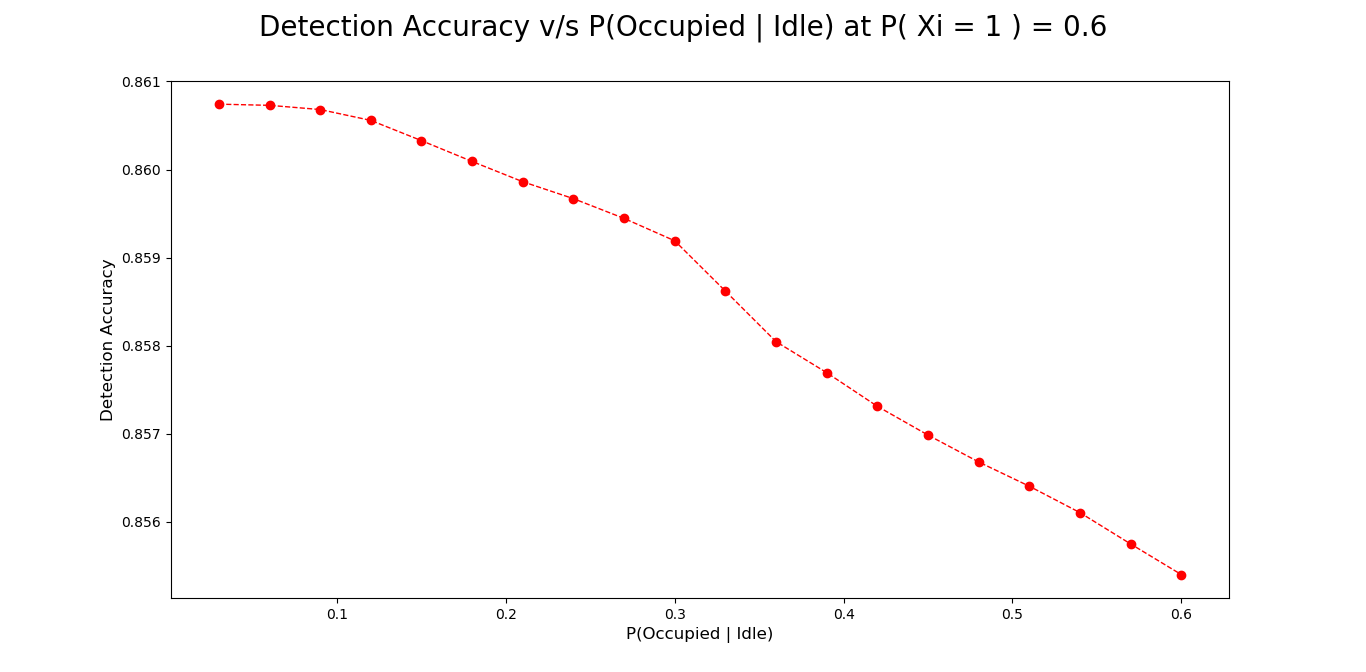
\includegraphics[width=1.0\textwidth]{Detection_Accuracy_vs_p_Iteration_1.png}
\caption{Detection Accuracy v/s $\mathbb P(Occupied|Idle)\ =\ p$ for a Double Markov chain Viterbi Estimator observing all 18 channels across 500 sampling rounds with Markovian correlation across channel indices and across time indices.}
\label{fig:mesh11}
\centering
\end{figure}
\section{Dynamic PU with Temporal Correlation and Channel Correlation with Incomplete Information}
\subsection{The Estimator}
In this extension, the SU does not sense all $|B|\ =\ K$ frequency bands in the wideband spectrum of interest. Instead, a subset $M\ <\ K$ frequency bands are sensed in a given sampling round based on recommendations given a Bandit or a Reinforcement Learning agent. Let the set of these "incomplete" observations in sampling round $t$ be given as,
\[\vec{Y}_t\ =\ [y_{t,1},\ y_{t,2},\ \phi,\ ...,\ \phi,....,\ y_{t,m},\ \phi,\ ...,\ y_{t,K}]^T\]
where, $\vec{Y}_t$ represents the observation vector in sampling round $t$ with $\phi$ filled in for frequency bands which have not been observed.
Based on this System Model and Observation Model, the state sequence estimation procedure detailed in Section 3 (\textit{Dynamic PU behavior with complete observations}) can be modified to account for missing observations as described below.
Persisting the same observation model and system model as in the previous sections, we can write the \textbf{Forward Recursion} step and \textbf{Backtracking} step of the 2D Viterbi algorithm with missing observations as follows,
\[V_{t,k}^{(r)}\ =\ m_r(y_{tk})max_{m,n}[a_{mnr}V_{t,k-1}^{(n)}V_{t-1,k}^{(m)}],\ if\ y_{tk}\neq\phi\]
\[V_{t,k}^{(r)}\ =\ max_{m,n}[a_{mnr}V_{t,k-1}^{(n)}V_{t-1,k}^{(m)}],\ if\ y_{tk}=\phi\]
\[x_{t-1,k-1}^*\ =\ l^*\ =\ argmax_{l}\{a_{mnr}\ V_{t,k-1}^{(n)}V_{t-1,k}^{(m)}\}\]
\subsection{Simulation Results}
The simulation parameters and methodologies are detailed below.
\begin{itemize}
    \item Number of channels in the wideband spectrum of interest = 18
    \item Number of sampling rounds / time indices = 1000
    \item Number of iterations / cycles to average out inconsistencies = 300
    \item Markovian correlation across both the time indices as well as the channel indices: The same model \[\theta\ =\ (A,\ B,\ \Pi)\] is used for both the chains.
    \item A customized Viterbi algorithm to account for missing information has been implemented in Python in order to verify the functionality of the proposed algorithm.
    \item A Channel Selection Strategy Generator has been implemented in Python to emulate a Channel Recommendation System such as an RL agent or a Multi-Armed Bandit.
    \item \[\mathbb P(Occupied\ |\ Idle)\ =\ p\ =\ \mathbb P(X_j=1\ |\ X_i=0)\] is varied from $0.03$ to \[\mathbb P(Occupied)\ =\ \mathbb P(X_i=1)\ =\ 0.6\] and the corresponding detection accuracies of the sensed and the un-sensed channels are plotted.
\end{itemize}
\section{DARPA SC2 DSRC Incumbent Spectrum Occupancy Behavior}
The Dynamic Short Range Communication (DSRC) Incumbent in a DARPA SC2 traffic scenario is modelled after a WLAN transceiver emulating PU-PU RF communications. The operational requirement of competitor radio nodes in a given DSRC scenario is that there should be no interference with the Incumbents' communications. The center frequency and bandwidth of the DSRC incumbent are not fixed and are not predefined. The competitor radio nodes should detect and workaround the Incumbents' spectrum occupancy behaviour.
\\As per the design specifications laid down in the SC2 website, the incumbent uses CSMA-based MAC along with OFDM and QPSK 1/2 modulation at the PHY layer. The incumbent used Layer-2 switching with ARP discovery for node-to-node traffic forwarding. Furthermore, the incumbent uses Layer3 routing protocols to advertise Colosseum traffic sub-nets among other incumbents.
\\The incumbents in the DSRC traffic scenario send out performance and location updates periodically to the competitor nodes over the collaboration network using the CIL message wrappers. The LocationUpdate CIL message contains latitude, longitude, and altitude information of the incumbent while the DetailedPerformance CIL message contains scalar\_performance, mandates\_achieved, hold\_period, and achieved\_duration parameters which are employed by the competitors to analyze the health/performance of the incumbent communications.
\\The following figures depict the Spectrum Occupancy Behavior of four Incumbents (SRN\_IDs: 111, 112, 113, and 114) across the scenario run-time in an SC2 DSRC reservation (Reservation\_ID: 72031). The radio.confs and colosseum\_config.ini files for these incumbents can be found on this projects GitHub repository (Minerva).
\begin{figure}[t]
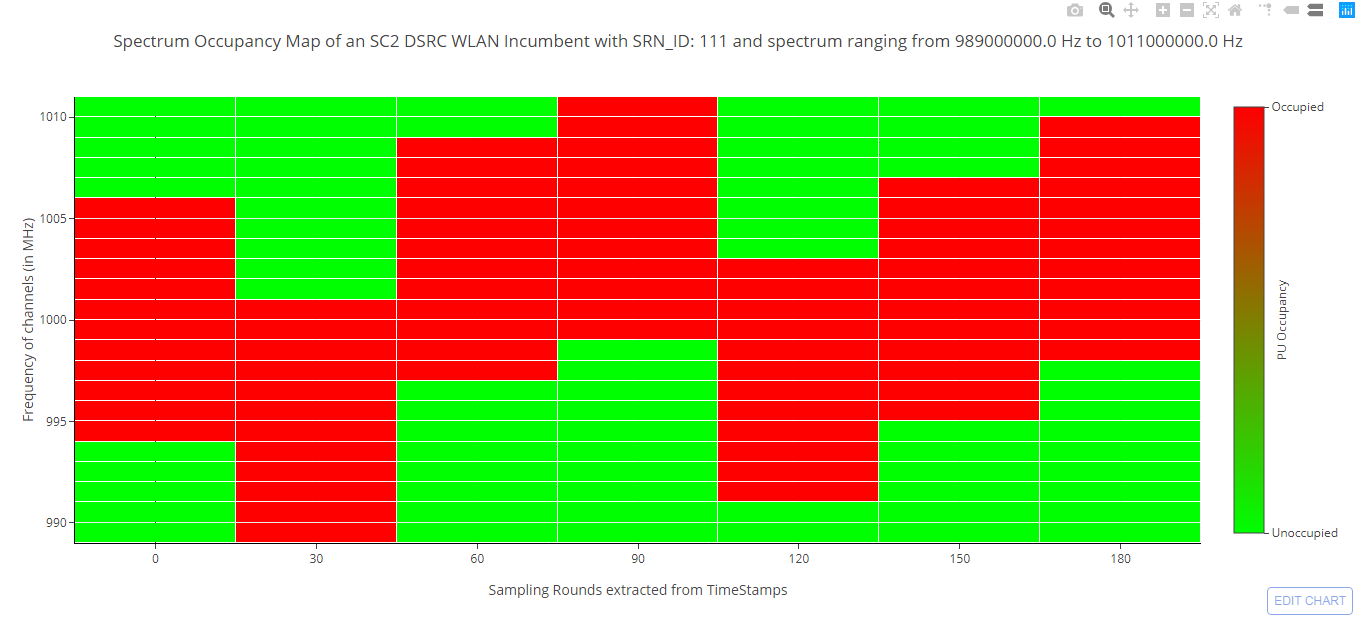
\includegraphics[width=1.0\textwidth]{Spectrum_Occupancy_DARPA_SC2_Incumbent_WLAN_DSRC_SRN_111.png}
\caption{Spectrum Occupancy Behavior of Incumbent 1 (SRN\_ID: 111) across the scenario run-time in SC2 DSRC traffic reservation 72031}
\label{fig:mesh12}
\centering
\end{figure}
\begin{figure}[t]
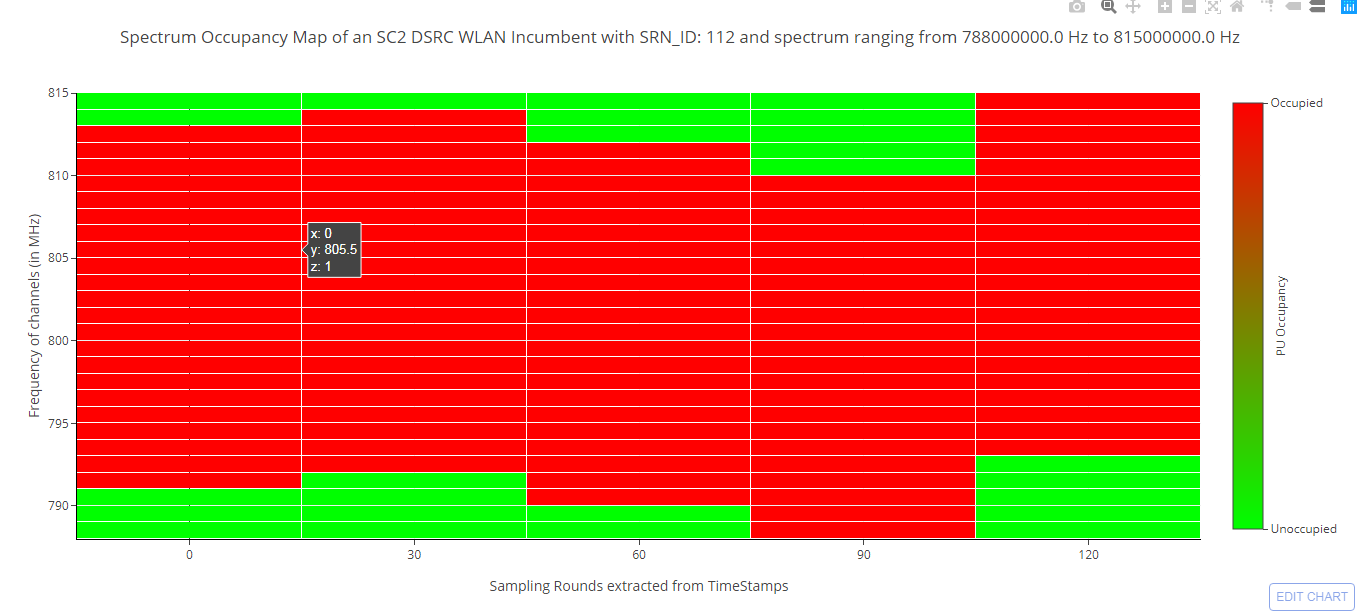
\includegraphics[width=1.0\textwidth]{Spectrum_Occupancy_DARPA_SC2_Incumbent_WLAN_DSRC_SRN_112.png}
\caption{Spectrum Occupancy Behavior of Incumbent 2 (SRN\_ID: 112) across the scenario run-time in SC2 DSRC traffic reservation 72031}
\label{fig:mesh13}
\centering
\end{figure}
\begin{figure}[t]
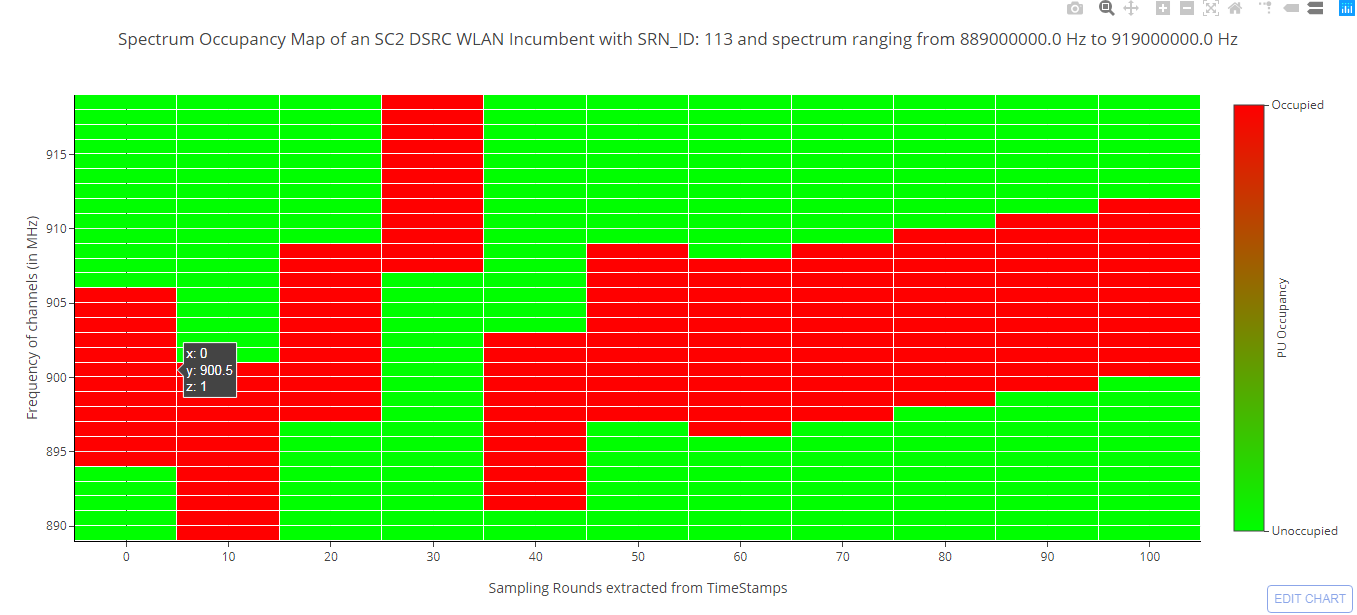
\includegraphics[width=1.0\textwidth]{Spectrum_Occupancy_DARPA_SC2_Incumbent_WLAN_DSRC_SRN_113.png}
\caption{Spectrum Occupancy Behavior of Incumbent 3 (SRN\_ID: 113) across the scenario run-time in SC2 DSRC traffic reservation 72031}
\label{fig:mesh14}
\centering
\end{figure}
\begin{figure}[t]
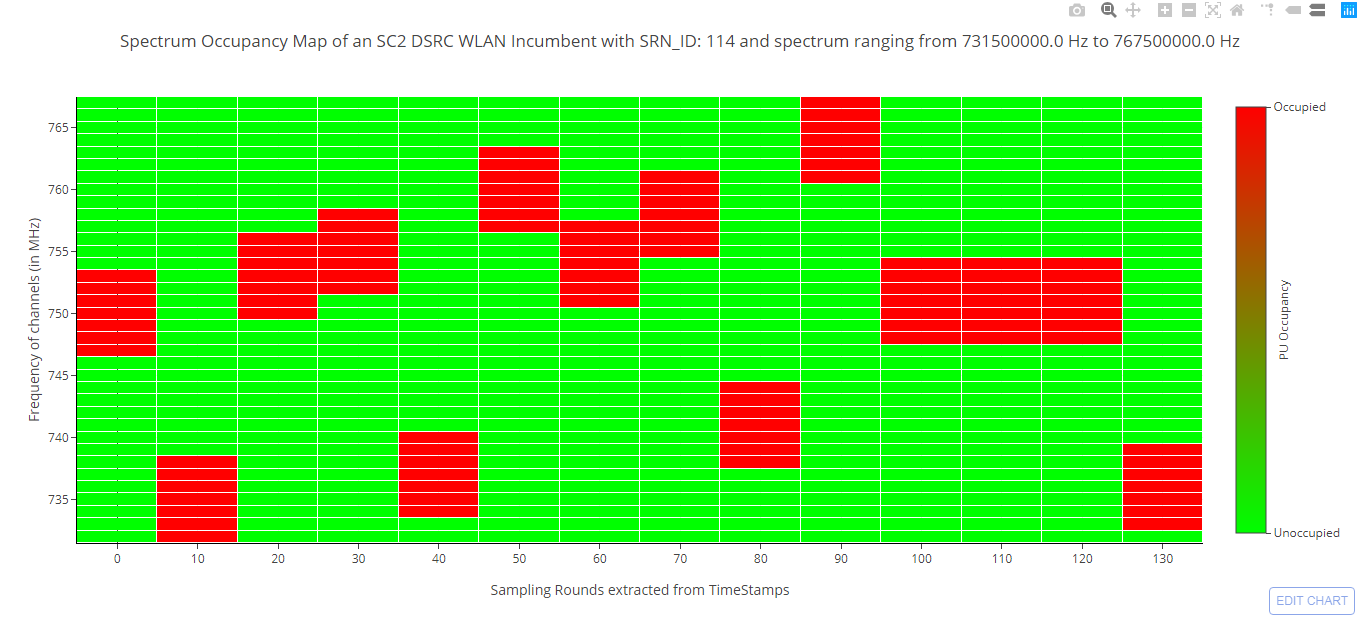
\includegraphics[width=1.0\textwidth]{Spectrum_Occupancy_DARPA_SC2_Incumbent_WLAN_DSRC_SRN_114.png}
\caption{Spectrum Occupancy Behavior of Incumbent 4 (SRN\_ID: 114) across the scenario run-time in SC2 DSRC traffic reservation 72031}
\label{fig:mesh15}
\centering
\end{figure}
\clearpage
\section{Markov Chain Parameter Estimation: Static PU with Markovian correlation across the channel indices with complete information}\label{VI}
\subsection{The Estimator}
Before diving into the algorithm, let us first define the Forward and Backward probabilities that will be employed in our estimation algorithm.
Let,
\[X_i\ =\ x_i\ be\ the\ PU\ Occupancy\ state\ of\ an\ arbitrary\ channel\]
\[X_{i+1}\ =\ X_j\ =\ x_j\ be\ the\ PU\ Occupancy\ state\ of\ the\ channel\ adjacent\ to\ channel\ b_i\]
\subsubsection{Forward Probabilities}
Let, $F(j,\ l)$ represent the probability of being in state $x_j=l$ after observing $y_1,\ y_2,\ y_3,\ ......,\ y_i,\ y_j$.
\begin{equation}\label{51}
    F(j,\ l)\ \triangleq \ \mathbb P(y_1,\ y_2,\ y_3,\ ....,\ y_i,\ y_j,\ x_j=l)
\end{equation}
Using the definition of Marginal Probability, equation (\ref{51}) can be written as,
\begin{equation}\label{52}
    F(j,\ l)\ = \ \sum_{r\in\{0,1\}}\ \mathbb P(y_1,\ y_2,\ y_3,\ ....,\ y_i,\ y_j,\ x_j=l,\ x_i=r)
\end{equation}
Using the definition of conditional probability, equation (\ref{52}) can be written as,
\begin{equation}\label{53}
    F(j,\ l)\ = \ \sum_{r\in\{0,1\}}\ \mathbb P(x_j=l,\ y_j\ |\ y_1,\ y_2,\ y_3,\ .....,\ y_i,\ x_i=r)\mathbb P(y_1,\ y_2,\ y_3,\ .....,\ y_i,\ x_i=r)
\end{equation}
Using the Markov property and definition of Forward Probability outlined in equation (\ref{51}), we can write equation (\ref{53}) as follows,
\begin{equation}\label{54}
    F(j,\ l)\ = \ \sum_{r\in\{0,1\}}\ \mathbb P(x_j=l,\ y_j\ |\ x_i=r)F(i,\ r)
\end{equation}
\subsubsection{Backward Probabilities}
Let $B(j,\ r)$ represent the probability of observing $y_j,\ y_{j+1},\ y_{j+2},\ ......,\ y_K$ given state $x_i\ =\ r$.
\begin{equation}\label{55}
    B(j,\ r)\ \triangleq\ \mathbb P(y_j,\ y_{j+1},\ y_{j+2},\ ......,\ y_K\ |\ x_i\ =\ r)
\end{equation}
Using the definition of Marginal Probabilities,
\begin{equation}\label{56}
    B(j,\ r)\ =\ \sum_{l\in\{0,1\}} \mathbb P(y_j,\ y_{j+1},\ y_{j+2},\ ......,\ y_K,\ x_j=l\ |\ x_i\ =\ r)
\end{equation}
Now, re-arranging the terms in equation (\ref{56}), we get,
\begin{equation}\label{57}
    B(j,\ r)\ =\ \sum_{l\in\{0,1\}} \mathbb P(y_{j+1},\ y_{j+2},\ ......,\ y_K,\ y_j,\ x_j=l\ |\ x_i\ =\ r)
\end{equation}
Now, we know that,
\begin{equation*}
    \mathbb P(A,\ B\ |\ C)\ =\ \mathbb P(A\ |\ B,\ C)\mathbb P(B\ |\ C)
\end{equation*}
Using this, we can write equation (\ref{57}) as,
\begin{equation}\label{58}
    B(j,\ r)\ =\ \sum_{l\in\{0,1\}} \mathbb P(y_{j+1},\ y_{j+2},\ ......,\ y_K\ |\ y_j,\ x_j=l,\ x_i\ =\ r)\mathbb P(y_j,\ x_j=l\ |\ x_i=r)
\end{equation}
Now, using the Markov property, equation (\ref{58}) can be written as,
\begin{equation}\label{59}
    B(j,\ r)\ =\ \sum_{l\in\{0,1\}} \mathbb P(y_{j+1},\ y_{j+2},\ ......,\ y_K\ |x_j=l)\mathbb P(y_j,\ x_j=l\ |\ x_i=r)
\end{equation}
Now, using the definition of Backward Probability outlined in equation (\ref{55}),
\begin{equation}\label{60}
    B(j,\ r)\ =\ \sum_{l\in\{0,1\}} B(j+1,\ l)\mathbb P(y_j,\ x_j=l\ |\ x_i=r)
\end{equation}
\subsubsection{Deriving the analytical expressions for the parameter estimation algorithm}
The HMM parameter estimation algorithm for our application can be derived using the Expectation-Maximization route.
\\The optimization objective is as follows,
\begin{equation}\label{61}
    A\ =\ argmax_{A}\ \mathbb{P}(\vec{y}\ |\ A)
\end{equation}
where,
\\$A$ is the state transition probability matrix
\[[A]_{lr}\ =\ a_{lr}\ =\ \mathbb{P}(x_j\ =\ r\ |\ x_i\ =\ l)\]
Converting this into an $argmax$ operation over log,
\begin{equation}\label{62}
    A\ =\ argmax_{A}\ log\ [\mathbb{P}(\vec{y}\ |\ A)]
\end{equation}
Using the definition of Marginal Probabilities,
\begin{equation}\label{63}
    A\ =\ argmax_{A}\ log\ [\sum_{\vec{x}}\ \mathbb{P}(\vec{x},\ \vec{y}\ |\ A)]
\end{equation}
This $argmax$ operation can be done over the joint probability distribution because the conditional is directly proportional to the joint as shown below.
\begin{equation}\label{64}
    A\ =\ argmax_{A}\ log\ [\sum_{\vec{x}}\ \mathbb{P}(\vec{x},\ \vec{y},\ A)]
\end{equation}
Explicitly specifying the summation range over the set of all possible state sequences,
\begin{equation}\label{65}
    A\ =\ argmax_{A}\ log\ [\sum_{k\ =\ 1}^{|X|}\ \mathbb{P}(\vec{x}_k,\ \vec{y},\ A)]
\end{equation}
where,
\[|X|\ =\ 2^{|B|}\ =\ 2^K\]
Multiply and divide by $\alpha_k$ where $0 \leq \alpha_k \leq 1$ and $\sum_{k}\ \alpha_k\ =\ 1$ in order to convert equation (\ref{65}) into a form of the Jensen's inequality.
\begin{equation}\label{66}
    A\ =\ argmax_{A}\ log\ [\sum_{k\ =\ 1}^{|X|}\ \alpha_k \frac{\mathbb{P}(\vec{x}_k,\ \vec{y},\ A)}{\alpha_k}]
\end{equation}
We know from Jensen's inequality that for any concave function $f(x)$, for any $x_i\ \in\ dom(f)\ (convex)$, and for any $0 \leq\ \theta_i\ \leq\ 1$ such that $\sum_i\ \theta_i\ =\ 1$,
\[f(\sum_i\ \theta_i x_i)\ \geq\ \sum_i\ \theta_i f(x_i)\]
Since the log function is concave, we can apply Jensen's inequality to equation (\ref{66}) as follows,
\begin{equation}\label{67}
    argmax_{A}\ log\ [\sum_{k\ =\ 1}^{|X|}\ \alpha_k \frac{\mathbb{P}(\vec{x}_k,\ \vec{y},\ A)}{\alpha_k}]\ \geq\ argmax_A\ \sum_{k=1}^{|X|}\ \alpha_k\ log\ [\frac{\mathbb{P}(\vec{x}_k,\ \vec{y},\ A)}{\alpha_k}]
\end{equation}
Now, $\alpha_k$ can be a Probability Mass Function because,
\[0\ \leq\ \alpha_k\ \leq\ 1\]
\[\sum_{k}\ \alpha_k\ =\ 1\]
Here, equation (\ref{67}) resembles,
\[f(\mathbb{E}[X])\ \geq\ \mathbb{E}[f(X)]\ for\ a\ concave\ function\ f(x)\]
The inequality holds only when $X$ is a degenerate random variable.
So, it is evident from equation (\ref{67}) that in order to ensure that equality holds, 
\begin{equation}\label{68}
    \frac{\mathbb{P}(\vec{x}_k,\ \vec{y},\ A)}{\alpha_k}\ =\ c\ with\ probability\ 1
\end{equation}
where, $c$ is a constant.
\\Therefore,
\begin{equation}\label{69}
    \alpha_k\ =\ \frac{\mathbb{P}(\vec{x}_k,\ \vec{y},\ A)}{c}
\end{equation}
We know that,
\[\sum_k\ \alpha_k\ =\ 1\]
Using this,
\begin{equation}\label{70}
    c\ =\ \sum_k\ \mathbb{P}(\vec{x}_k,\ \vec{y},\ A)
\end{equation}
Now, using these results,
\begin{equation}\label{71}
    \alpha_k\ =\ \frac{\mathbb{P}(\vec{x}_k,\ \vec{y},\ A)}{\sum_k\ \mathbb{P}(\vec{x}_k,\ \vec{y},\ A)}
\end{equation}
Using the definition of Marginal Probabilities,
\begin{equation}\label{72}
    \alpha_k\ =\ \frac{\mathbb{P}(\vec{x}_k,\ \vec{y},\ A)}{\mathbb{P}(\vec{y},\ A)}\ =\ \mathbb{P}(\vec{x}_k\ |\ \vec{y},\ A)
\end{equation}
So, now the optimization problem becomes,
\begin{equation}\label{73}
    A\ =\ argmax_A\ \sum_{k\ =\ 1}^{|X|}\ \mathbb{P}(\vec{x}_k\ |\ \vec{y},\ \hat{A})\ log\ [\frac{\mathbb{P}(\vec{x}_k,\ \vec{y},\ A)}{\mathbb{P}(\vec{x}_k\ |\ \vec{y},\ \hat{A})}]
\end{equation}
Here, $\hat{A}$ is the previous estimate of the state transition probability matrix [This will turn out to be an iterative algorithm, i.e. the evaluation and re-estimation repeats until suitable convergence].
We don't care about the denominator in the above optimization problem,
\begin{equation}\label{74}
    A\ =\ argmax_A\ \sum_{k\ =\ 1}^{|X|}\ \mathbb{P}(\vec{x}_k\ |\ \vec{y},\ \hat{A})\ log\ [\mathbb{P}(\vec{x}_k,\ \vec{y},\ A)]
\end{equation}
Using the HMM System Model,
\begin{equation}\label{75}
    A\ =\ argmax_A\ \sum_{k\ =\ 1}^{|X|}\ \mathbb{P}(\vec{x}_k\ |\ \vec{y},\ \hat{A})\ log\ [\prod_{i\ =\ 1}^K\ \mathbb{P}(y_i\ |\ x_i)\ \mathbb{P}(x_i\ |\ x_{i-1},\ \hat{A})]
\end{equation}
where, if $i\ =\ 1$,
\[\mathbb{P}(x_i\ |\ x_{i-1},\ \hat{A})\ =\ \mathbb{P}(X_1\ =\ x_1)\]
Using the properties of logarithms,
\begin{equation}\label{76}
    A\ =\ argmax_A\ \sum_{k\ =\ 1}^{|X|}\ \mathbb{P}(\vec{x}_k\ |\ \vec{y},\ \hat{A})\ \sum_{i\ =\ 1}^K\ log\ [\mathbb{P}(y_i\ |\ x_i)]\ +\ log\ [\mathbb{P}(x_i\ |\ x_{i-1},\ \hat{A})]
\end{equation}
Using indicator random variables to expand the state and observation associations,
\begin{equation}\label{77}
    \begin{aligned}
        A\ =\ argmax_A\ \sum_{k\ =\ 1}^{|X|}\ \mathbb{P}(\vec{x}_k\ |\ \vec{y},\ \hat{A})\ \sum_{l\ \in\ \{0,\ 1\}}\ \sum_{r\ \in\ \{0,\ 1\}}\ \sum_{i\ =\ 1}^{K}\ \sum_{j\ =\ 1}^{K}\ I\{x_i\ =\ r\ and\ y_j\ =\ y_i\}\ log\ [m_r(y_i)]\ \\+\ I\{x_{i-1}\ =\ l\ and\ x_i\ =\ r\}\ log\ [a_{lr}]
    \end{aligned}
\end{equation}
Using Lagrange multipliers to find the solution, the Lagrangian is given as follows,
\begin{equation}\label{78}
    \begin{aligned}
        \mathcal{L}\ =\ \sum_{k\ =\ 1}^{|X|}\ \mathbb{P}(\vec{x}_k\ |\ \vec{y},\ \hat{A})\ \sum_{l\ \in\ \{0,\ 1\}}\ \sum_{r\ \in\ \{0,\ 1\}}\ \sum_{i\ =\ 1}^{K}\ \sum_{j\ =\ 1}^{K}\ I\{x_i\ =\ r\ and\ y_j\ =\ y_i\}\ log\ [m_r(y_i)]\ +\ \\I\{x_{i-1}\ =\ l\ and\ x_i\ =\ r\}\ log\ [a_{lr}]\ +\ \sum_{l\ \in\ \{0,\ 1\}}\ \lambda_i(1-\sum_{r\ \in\ \{0,\ 1\}}\ a_{lr})
    \end{aligned}
\end{equation}
Differentiating with respect to $a_{lr}$ and equating it to 0,
\begin{equation}\label{79}
    \frac{\partial}{\partial a_{lr}}\mathcal{L}\ =\ \sum_{k\ =\ 1}^{|X|}\ \mathbb{P}(\vec{x}_k\ |\ \vec{y},\ \hat{A})\ \frac{1}{a_{lr}}\sum_{i\ =\ 1}^{K}\ I\{x_{i-1}\ =\ l\ and\ x_i\ =\ r\}\ -\ \lambda_i\ =\ 0
\end{equation}
Simplifying this, we get,
\begin{equation}\label{80}
    a_{lr}\ =\ \frac{1}{\lambda_i} \sum_{k\ =\ 1}^{|X|}\ \mathbb{P}(\vec{x}_k\ |\ \vec{y},\ \hat{A}) \sum_{i\ =\ 1}^{K}\ I\{x_{i-1}\ =\ l\ and\ x_i\ =\ r\}
\end{equation}
Differentiating with respect to our Lagrange multiplier $\lambda_i$ and equating it to 0,
\begin{equation}\label{81}
    \frac{\partial}{\partial \lambda_i}\mathcal{L}\ =\ (1-\sum_{r\ \in\ \{0,\ 1\}}\ a_{lr}) =\ 0
\end{equation}
Simplifying this using equation (\ref{80}), we get,
\begin{equation}\label{82}
    \lambda_i\ =\ \sum_{r\ \in\ \{0,\ 1\}}\ \sum_{k\ =\ 1}\ \mathbb{P}(\vec{x}\ |\ \vec{y},\ \hat{A})\ \sum_{i\ =\ 1}^{K}\ I\{x_{i-1}\ =\ l\ and\ x_i\ =\ r\}
\end{equation}
Using the definition of Marginal Probabilities, we can write equation (\ref{82}) as follows,
\begin{equation}\label{83}
    \lambda_i\ =\ \sum_{k\ =\ 1}^{|X|}\ \mathbb{P}(\vec{x}\ |\ \vec{y},\ \hat{A})\ \sum_{i\ =\ 1}^{K}\ I\{x_{i-1}\ =\ l\}
\end{equation}
Using equation (\ref{83}) in equation (\ref{80}), we get,
\begin{equation}\label{84}
    a_{lr}\ =\ \frac{\sum_{k\ =\ 1}^{|X|}\ \mathbb{P}(\vec{x}_k\ |\ \vec{y},\ \hat{A}) \sum_{i\ =\ 1}^{K}\ I\{x_{i-1}\ =\ l\ and\ x_i\ =\ r\}}{\sum_{k\ =\ 1}^{|X|}\ \mathbb{P}(\vec{x}\ |\ \vec{y},\ \hat{A})\ \sum_{i\ =\ 1}^{K}\ I\{x_{i-1}\ =\ l\}}
\end{equation}
Let's simplify equation (\ref{84}) further to remove the summation over all possible state sequences,
\begin{equation}\label{85}
    a_{lr}\ =\ \frac{\sum_{k\ =\ 1}^{|X|}\ \sum_{i\ =\ 1}^{K}\ \mathbb{P}(\vec{x}_k\ |\ \vec{y},\ \hat{A})\ I\{x_{i-1}\ =\ l\ and\ x_i\ =\ r\}}{\sum_{k\ =\ 1}^{|X|}\ \sum_{i\ =\ 1}^{K}\ \mathbb{P}(\vec{x}\ |\ \vec{y},\ \hat{A})\ I\{x_{i-1}\ =\ l\}}
\end{equation}
Using the definition of Conditional Probability,
\begin{equation}\label{86}
    a_{lr}\ =\ \frac{\sum_{k\ =\ 1}^{|X|}\ \sum_{i\ =\ 1}^{K}\ \mathbb{P}(\vec{x}_k,\ \vec{y},\ \hat{A})\ I\{x_{i-1}\ =\ l\ and\ x_i\ =\ r\}}{\sum_{k\ =\ 1}^{|X|}\ \sum_{i\ =\ 1}^{K}\ \mathbb{P}(\vec{x},\ \vec{y},\ \hat{A})\ I\{x_{i-1}\ =\ l\}}
\end{equation}
Combining the Indicator with the Joint,
\begin{equation}\label{87}
    a_{lr}\ =\ \frac{\sum_{k\ =\ 1}^{|X|}\ \sum_{i\ =\ 1}^{K}\ \mathbb{P}(\vec{x}_k,\ \vec{y},\ \hat{A},\ x_{i-1}\ =\ l,\ x_i\ =\ r)}{\sum_{k\ =\ 1}^{|X|}\ \sum_{i\ =\ 1}^{K}\ \mathbb{P}(\vec{x},\ \vec{y},\ \hat{A},\ x_{i-1}\ =\ l)}
\end{equation}
Using the definition of Marginal Probabilities,
\begin{equation}\label{88}
    a_{lr}\ =\ \frac{\sum_{i\ =\ 1}^{K}\ \mathbb{P}(\vec{y},\ \hat{A},\ x_{i-1}\ =\ l,\ x_i\ =\ r)}{\sum_{i\ =\ 1}^{K}\ \mathbb{P}(\vec{y},\ \hat{A},\ x_{i-1}\ =\ l)}
\end{equation}
Expanding the observation vector and using the definition of Marginal Probabilities to modify the denominator,
\begin{equation}\label{89}
    a_{lr}\ =\ \frac{\sum_{i\ =\ 1}^{K}\ \mathbb{P}(y_1,\ y_2,\ ....,\ y_{i-1},\ x_{i-1}\ =\ l,\ y_i,\ x_i\ =\ r,\ y_{i+1},\ y_{i+2},\ ....,\ y_K,\ \hat{A})}{\sum_{r\ \in\ \{0,\ 1\}}\ \sum_{i\ =\ 1}^{K}\ \mathbb{P}(y_1,\ y_2,\ ....,\ y_{i-1},\ x_{i-1}\ =\ l,x_i\ =\ r,\ y_i,\ y_{i+1},\ y_{i+2},\ ....,\ y_K,\ \hat{A})}
\end{equation}
Extracting the independent terms and creating conditionals,
\begin{equation}\label{90}
    \begin{aligned}
        a_{lr}\ =\ \frac{\sum_{i=1}^{K}\mathbb{P}(y_1,..,y_{i-1},x_{i-1}=l)\mathbb{P}(y_i,x_i=r|y_1,..,y_{i-1},x_{i-1}=l,\hat{A})\mathbb{P}(y_{i+1},..,y_K|x_i=r)}{\sum_{r\in\{0,1\}}\sum_{i=1}^{K}\mathbb{P}(y_1,..,y_{i-1},x_{i-1}=l)\mathbb{P}(x_i=r,y_i|y_1,..,y_{i-1},x_{i-1}=l,\hat{A})\mathbb{P}(y_{i+1},..,y_K|x_i=r)}
    \end{aligned}
\end{equation}
Using the properties of the assumed Markov Chain model,
\begin{equation}\label{91}
    \begin{aligned}
        a_{lr}\ =\ \frac{\sum_{i=1}^{K}\mathbb{P}(y_1,..,y_{i-1},x_{i-1}=l)\mathbb{P}(y_i,x_i=r|x_{i-1}=l,\hat{A})\mathbb{P}(y_{i+1},..,y_K|x_i=r)}{\sum_{r\in\{0,1\}}\sum_{i=1}^{K}\mathbb{P}(y_1,..,y_{i-1},x_{i-1}=l)\mathbb{P}(x_i=r,y_i|x_{i-1}=l,\hat{A})\mathbb{P}(y_{i+1},..,y_K|x_i=r)}
    \end{aligned}
\end{equation}
Now, we know that,
\[P(y_i,\ x_i\ =\ r\ |\ x_{i-1}\ =\ l,\ \hat{A})\ =\ m_r(y_i)a_{lr}\]
Using this to re-write equation (\ref{92}),
\begin{equation}\label{92}
    \begin{aligned}
        a_{lr}\ =\ \frac{\sum_{i=1}^{K}\mathbb{P}(y_1,..,y_{i-1},x_{i-1}=l)m_r(y_i)a_{lr}\mathbb{P}(y_{i+1},..,y_K|x_i=r)}{\sum_{r\in\{0,1\}}\sum_{i=1}^{K}\mathbb{P}(y_1,..,y_{i-1},x_{i-1}=l)m_r(y_i)a_{lr}\mathbb{P}(y_{i+1},..,y_K|x_i=r)}
    \end{aligned}
\end{equation}
We know from our definitions of Forward and Backward Probabilities defined in equations (\ref{51}) and (\ref{55}) respectively that,
\[\mathbb{P}(y_1,..,y_{i-1},x_{i-1}=l)\ =\ F(i-1,\ l)\]
\[\mathbb{P}(y_{i+1},..,y_K|x_i=r)\ =\ B(i+1,\ r)\]
Using these results in equation (\ref{92}),
\begin{equation}\label{93}
    \begin{aligned}
        a_{lr}\ =\ \frac{\sum_{i=1}^{K}F(i-1,l)m_r(y_i)a_{lr}B(i+1,r)}{\sum_{r\in\{0,1\}}\sum_{i=1}^{K}F(i-1,l)m_r(y_i)a_{lr}B(i+1,r)}
    \end{aligned}
\end{equation}
\subsection{The Algorithm}
\textbf{Known Parameters}: 
\begin{itemize}
    \item Variance of the channel impulse response, i.e. $\sigma_H^2$
    \item Variance of the noise, i.e. $\sigma_V^2$
    \item Emission Probabilities = $m_l(y_i)\ \sim \mathcal{CN}(0,\ \sigma_H^2 l + \sigma_V^2)$
\end{itemize}
\textbf{Initialization}: Initialize the state transition probability matrix $(A)$ to some random values.
\[\mathbb{P}(X_1\ =\ 1)\ =\ \Pi\]
\[a_{lr}\ =\ \mathbb{P}(x_j\ =\ r\ |\ x_i\ =\ l)\]
\textbf{Iteration}: Evaluate the Forward and Backward probabilities using current estimates of $A$, the state transition probability matrix.
\[F(i-1,\ l)^{t}\ = \ \sum_{k\in\{0,1\}}\ m_l(y_{i-1})a_{kl}^tF(i-2,\ k)\]
\[B(i+1,\ r)^{t}\ =\ \sum_{s\in\{0,1\}}\ m_s(y_{i+2})a_{rs}^tB(i+2,\ s)\]
Re-estimate the elements of the state transition probability matrix.
\[a_{lr}^{t+1}\ =\ \frac{\sum_{i=1}^{K}F(i-1,l)^{t}m_r(y_i)a_{lr}^{t}B(i+1,r)^{t}}{\sum_{r\in\{0,1\}}\sum_{i=1}^{K}F(i-1,l)^{t}m_r(y_i)a_{lr}^{t}B(i+1,r)^{t}}\]
\textbf{Termination}: 
\[|a_{lr}^{t+1}\ -\ a_{lr}^t| \leq \epsilon\]
where,
$t$ is the iteration counter, $\forall\ l,\ r\ \in\ \{0,\ 1\}$, and for any $\epsilon > 0$
\subsection{Simulation Results}
The algorithm outlined in the previous subsection has been implemented in Python and its results are detailed in this subsection.
\begin{itemize}
    \item Number of frequency bands / channels = 18
    \item Number of observation vectors = 300
    \item SNR (signal ON) = 19.03 dB
    \item Convergence Threshold ($\epsilon$) = $10^{-5}$
    \item Initial Assignment of $\mathbb{P}(Occupied\ |\ Idle)\ =\ p$ = $10^{-5}$
    \item True value of $\mathbb{P}(Occupied\ |\ Idle)\ =\ p$ = 0.30
    \item Convergence repeat (confidence) threshold = 7
\end{itemize}
For an actual value of
\[\mathbb{P}(Occupied\ |\ Idle)\ =\ p\ =\ 0.30\]
and starting with an initial random assignment of $\hat{p}\ =\ 10^{-5}$, we see that the Markov Chain Parameter Estimator algorithm in the previous subsection converges to a value of $\hat{p}\ =\ 0.2922942008349906$ in 150 iterations across 300 observation vectors.
\\A plot of $Mean\ Square\ Error\ =\ \mathbb{E}[(p\ -\ \hat{p})^2]$ versus the $Number\ of\ Iterations$ is shown in Figure 16 for the algorithm described in the previous subsection.
\begin{figure}[t]
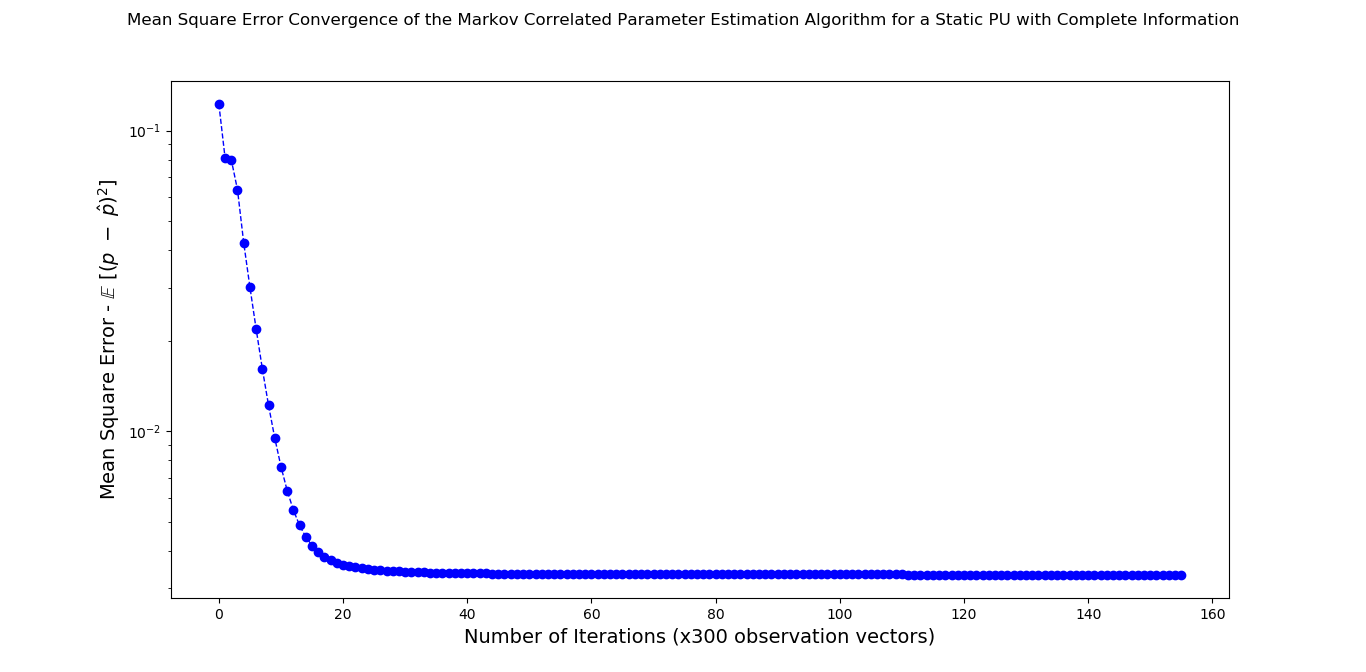
\includegraphics[width=1.0\textwidth]{Mean_Square_Plot_Log_Scale.png}
\caption{Mean Square Error v/s Number of Iterations - A plot of convergence of our variant of EM for HMMs in order to estimate the parameters of the Markov Chain.}
\label{fig:mesh16}
\centering
\end{figure}
\section{Modelling the SU Spectrum Access Behavior as a Partially Observable Markov Decision Process (POMDP)}
\subsection{POMDP Agent Model}
Partially Observable Markov Decision Processes (POMDPs) model the repeated interactions of an agent with a stochastic environment, parts of which are hidden (un-observable or observable with noise or both) from the agent's view, in order to maximize the utility of a specific task.
\\The following are important points to note about POMDPs in general and the POMDP model used in this work.
\begin{itemize}
    \item The agent's role is to perform tasks by choosing \textbf{actions} that fulfill the given task(s) in the best possible way.
    \item The run-time or the interaction-time of the POMDP is quantized into discrete time-steps termed \textbf{episodes} and the agent executes an action at the start of each time-step.
    \item Upon executing an action, the agent receives a scalar parameter value termed the \textbf{reward} from the environment and the goal of the agent is to maximize the long-term cumulative (finite-horizon or infinite horizon) reward it can get.
    \item The agent's limited observational capabilities and/or the agent's noisy observations result in a level of uncertainty at the agent's end regarding the \textbf{state} of the environment and the exact effect of executing an action on the environment.
    \item Notations: \begin{itemize}
        \item $\mathcal{X}$ denotes the finite, discrete \textbf{State Space} and $\vec{x} \in \mathcal{X}$ represents an element of this space
        \item $\mathcal{A}$ denotes the finite, discrete \textbf{Action Space} and $a \in \mathcal{A}$ represents an element of this space
        \item $\mathcal{Y}$ denotes the continuous \textbf{Observation Space} and $\vec{y} \in \mathcal{Y}$ represents an element of this space
    \end{itemize}
    \item The \textbf{Transition Model} of the POMDP, i.e. $\mathbb{P}(\vec{x}'|\vec{x},\ a)$ is unknown and will be learnt during interactions using the Parameter Estimation Algorithm detailed in Section \ref{VI}.
    \item The \textbf{Emission Model} of the POMDP, i.e. $\mathbb{P}(\vec{y}|\vec{x},\ a)$ is given from the System Model and Observation Model detailed in the previous sections of this work.
    \item Given the POMDP Transition model (learnt over time) and the POMDP Emission model (known from the assumed System Model and the assumed Observation Model), the POMDP for SU spectrum access behavior in the presence of a PU can be converted to a \textbf{Belief state MDP}.
    \item The POMDP agent assumes an initial belief $\vec{b}_0$ where, $\mathbb{P}(\vec{b}_0)\ =\ \frac{1}{|\mathcal{X}|}$, i.e. Uniform distribution over the State Space.
    \item At the beginning of each episode, the agent takes an action $a \in \mathcal{A}$, observes $\vec{y} \in \mathcal{Y}$, and updates its belief as follows.
    \[b_a^{\vec{y}}(\vec{x}')\ =\ \mathbb{P}(\vec{x}'|\vec{y},\ a,\ \vec{b})\]
    Using the definition of Conditional Probability,
    \[b_a^{\vec{y}}(\vec{x}')\ =\ \frac{\mathbb{P}(\vec{x}',\ \vec{y},\ a,\ \vec{b})}{\mathbb{P}(\vec{y},\ a,\ \vec{b})}\ =\ \frac{\mathbb{P}(\vec{y}|\vec{x}',\ a,\ \vec{b})\mathbb{P}(\vec{x}',\ a,\ \vec{b})}{\mathbb{P}(\vec{y},\ a,\ \vec{b})}\]
    Using the definition of Marginal Probability,
    \[b_a^{\vec{y}}(\vec{x}')\ =\ \frac{\mathbb{P}(\vec{y}|\vec{x}',\ a,\ \vec{b})\sum_{\vec{x} \in \mathcal{X}}\ \mathbb{P}(\vec{x},\ \vec{x}',\ a,\ \vec{b})}{\mathbb{P}(\vec{y}|a,\ \vec{b})\mathbb{P}(a,\ \vec{b})}\]
    Again, using the definition of Conditional Probability,
    \[b_a^{\vec{y}}(\vec{x}')\ =\ \frac{\mathbb{P}(\vec{y}|\vec{x}',\ a,\ \vec{b})\sum_{\vec{x} \in \mathcal{X}}\ \mathbb{P}(\vec{x}'|\vec{x},\ a,\ \vec{b})\mathbb{P}(\vec{x},\ a,\ \vec{b})}{\mathbb{P}(\vec{y}|a,\ \vec{b})\mathbb{P}(a,\ \vec{b})}\]
    Since the state transitions of the environment and the agent's observations of the environment do not depend on the agent's belief $\vec{b}$ given the action executed $a$,
    \[b_a^{\vec{y}}(\vec{x}')\ =\ \frac{\mathbb{P}(\vec{y}|\vec{x}',\ a)\sum_{\vec{x} \in \mathcal{X}}\ \mathbb{P}(\vec{x}'|\vec{x},\ a)\mathbb{P}(\vec{x}|a,\ \vec{b})\mathbb{P}(a,\ \vec{b})}{\mathbb{P}(\vec{y}|a,\ \vec{b})\mathbb{P}(a,\ \vec{b})}\]
    Re-arranging,
    \[b_a^{\vec{y}}(\vec{x}')\ =\ \frac{\mathbb{P}(\vec{y}|\vec{x}',\ a)}{\mathbb{P}(\vec{y}|a,\ \vec{b})}\sum_{\vec{x} \in \mathcal{X}}\ \mathbb{P}(\vec{x}'|\vec{x},\ a)\mathbb{P}(\vec{x}|a,\ \vec{b})\]
    where,
    \\$b(\vec{x})\ =\ \mathbb{P}(\vec{x}|a,\ \vec{b})$ is the probability (degree of certainty or "belief") assigned to world state $\vec{x} \in \mathcal{X}$ by belief state $\vec{b}$
    \\Note here that $b(\vec{x})$ like any valid probability measure satisfies the Kolmogorav's axioms as shown below.
    \[\sum_{\vec{x} \in \mathcal{X}}\ b(\vec{x})\ =\ 1\]
    \[0 \leq b(\vec{x}) \leq 1\]
    Finally,
    \[b_a^{\vec{y}}(\vec{x}')\ =\ \frac{\mathbb{P}(\vec{y}|\vec{x}',\ a)}{\mathbb{P}(\vec{y}|a,\ \vec{b})}\sum_{\vec{x} \in \mathcal{X}}\ \mathbb{P}(\vec{x}'|\vec{x},\ a)b(\vec{x})\]
    The denominator $\mathbb{P}(\vec{y}|a,\ \vec{b})$ needs to be described using the POMDP's Transition Model and Emission Model. This is done as shown below.
    \[\mathbb{P}(\vec{y}|a,\ \vec{b})\ =\ \frac{\mathbb{P}(\vec{y},\ a,\ \vec{b})}{\mathbb{P}(a,\ \vec{b})}\]
    Using the definition of Marginal Probability,
    \[\mathbb{P}(\vec{y}|a,\ \vec{b})\ =\ \frac{\sum_{\vec{x}' \in \mathcal{X}}\ \mathbb{P}(\vec{x}',\ \vec{y},\ a,\ \vec{b})}{\mathbb{P}(a,\ \vec{b})}\]
    Now, using the definition of Conditional Probability in order to bring out the POMDP's Emission Model,
    \[\mathbb{P}(\vec{y}|a,\ \vec{b})\ =\ \frac{\sum_{\vec{x}' \in \mathcal{X}}\ \mathbb{P}(\vec{y}|\vec{x}',\ a,\ \vec{b})\mathbb{P}(\vec{x}',\ a,\ \vec{b})}{\mathbb{P}(a,\ \vec{b})}\]
    Using the definition of Marginal Probability and Removing the independent variables from the terms, we get,
    \[\mathbb{P}(\vec{y}|a,\ \vec{b})\ =\ \frac{\sum_{\vec{x}' \in \mathcal{X}}\ \mathbb{P}(\vec{y}|\vec{x}',\ a)\sum_{\vec{x} \in \mathcal{X}}\ \mathbb{P}(\vec{x},\ \vec{x}',\ a,\ \vec{b})}{\mathbb{P}(a,\ \vec{b})}\]
    Now, using the definition of Conditional Probability in order to bring in the POMDP's Transition Model,
    \[\mathbb{P}(\vec{y}|a,\ \vec{b})\ =\ \frac{\sum_{\vec{x}' \in \mathcal{X}}\ \mathbb{P}(\vec{y}|\vec{x}',\ a)\sum_{\vec{x} \in \mathcal{X}}\ \mathbb{P}(\vec{x}'|\vec{x},\ a,\ \vec{b})\mathbb{P}(a,\ \vec{b},\ \vec{x})}{\mathbb{P}(a,\ \vec{b})}\]
    Since environment state transitions do not depend on the POMDP agent's beliefs,
    \[\mathbb{P}(\vec{y}|a,\ \vec{b})\ =\ \frac{\sum_{\vec{x}' \in \mathcal{X}}\ \mathbb{P}(\vec{y}|\vec{x}',\ a)\sum_{\vec{x} \in \mathcal{X}}\ \mathbb{P}(\vec{x}'|\vec{x},\ a)\mathbb{P}(a,\ \vec{b},\ \vec{x})}{\mathbb{P}(a,\ \vec{b})}\]
    Simplifying further,
    \[\mathbb{P}(\vec{y}|a,\ \vec{b})\ =\ \frac{\sum_{\vec{x}' \in \mathcal{X}}\ \mathbb{P}(\vec{y}|\vec{x}',\ a)\sum_{\vec{x} \in \mathcal{X}}\ \mathbb{P}(\vec{x}'|\vec{x},\ a)\mathbb{P}(\vec{x}|a,\ \vec{b})\mathbb{P}(a,\ \vec{b})}{\mathbb{P}(a,\ \vec{b})}\]
    \[\mathbb{P}(\vec{y}|a,\ \vec{b})\ =\ \sum_{\vec{x}' \in \mathcal{X}}\ \mathbb{P}(\vec{y}|\vec{x}',\ a)\sum_{\vec{x} \in \mathcal{X}}\ \mathbb{P}(\vec{x}'|\vec{x},\ a)\mathbb{P}(\vec{x}|a,\ \vec{b})\]
    But, as we saw earlier, $\mathbb{P}(\vec{x}|a,\ \vec{b})\ =\ b(\vec{x})$,
    \[\mathbb{P}(\vec{y}|a,\ \vec{b})\ =\ \sum_{\vec{x}' \in \mathcal{X}}\ \mathbb{P}(\vec{y}|\vec{x}',\ a)\sum_{\vec{x} \in \mathcal{X}}\ \mathbb{P}(\vec{x}'|\vec{x},\ a)b(\vec{x})\]
    Combining these results, the belief update step is outlined below.
    \begin{equation}\label{94}
        b_a^{\vec{y}}(\vec{x}')\ =\ \frac{\mathbb{P}(\vec{y}|\vec{x}',\ a)}{\mathbb{P}(\vec{y}|a,\ \vec{b})}\sum_{\vec{x} \in \mathcal{X}}\ \mathbb{P}(\vec{x}'|\vec{x},\ a)b(\vec{x})
    \end{equation}
    where,
    \begin{equation}\label{95}
        \mathbb{P}(\vec{y}|a,\ \vec{b})\ =\ \sum_{\vec{x}' \in \mathcal{X}}\ \mathbb{P}(\vec{y}|\vec{x}',\ a)\sum_{\vec{x} \in \mathcal{X}}\ \mathbb{P}(\vec{x}'|\vec{x},\ a)b(\vec{x})
    \end{equation}
    \item The \textbf{action policy} denoted by $\pi: \mathcal{B} \rightarrow \mathcal{A}$ maps the beliefs $\vec{b} \in \mathcal{B}$ to actions $a \in \mathcal{A}$ in order to satisfy the agent's goal of maximizing the cumulative long-term reward associated with the fulfillment of the given task.
    \item The \textbf{belief-space} is an $|\mathcal{X}|-1$ dimensional simplex.
    \\NOTE: An $n$-simplex is an n-dimensional polytope which is the convex-hull of its $(n+1)$ vertices.
    \item A policy $\pi$ is characterized by a \textbf{value function} $V^{\pi}: \mathcal{B} \rightarrow \mathbb{R}$ which is defined as the expected discounted future reward $V^{\pi}(\vec{b})$ the agent can accumulate by following policy $\pi$ starting from belief $\vec{b}$.
    \begin{equation}\label{96}
        V^{\pi}(\vec{b})\ =\ \mathbb{E}_{\pi}\Big[\sum_{t=0}^{\infty}\ \gamma^t R(\vec{b}_t,\ \pi(\vec{b}_t))|\vec{b}_0=\vec{b}\Big]
    \end{equation}
    where,
    \begin{equation}\label{97}
       R(b_t,\ \pi(\vec{b}_t)\ =\ \sum_{\vec{x} \in \mathcal{X}}\ R(\vec{x},\ \pi(\vec{b}_t))b_t(\vec{x})
    \end{equation}
    Furthermore, here,
    \\$R(\vec{b}_t,\ \pi(\vec{b}_t))\ \triangleq\ $The average / expected reward for policy $\pi$ and belief $\vec{b}_t$,
    \\$R(\vec{x},\ \pi(\vec{b}_t))\ \triangleq\ $The world reward for state $\vec{x} \in \mathcal{X}$ and action $a\ =\ \pi(\vec{b}_t) \in \mathcal{A}$,
    \\$b_t(\vec{x})$ is the "belief" of being in state $\vec{x}$, and
    \\$\gamma\ \triangleq\ $The discount factor such that $0 < \gamma < 1$.
    \item Before we jump into evaluating or solving for an optimal policy, let's define a \textbf{policy tree}. A policy tree is a complete $t$-step \textbf{non-stationary policy} for \textbf{finite-horizon POMDPs}.
    \item The \textbf{optimal policy} $\pi^*$ specifies the optimal action to execute in the current episode, assuming the POMDP agent acts optimally in future episodes too. Let's derive a mathematical expression for the value function of the optimal policy at a particular belief state $\vec{b} \in \mathcal{B}$ as follows.
    \\For a 1-step policy tree $p$,
    \[V_p(\vec{b})\ =\ R(\vec{b},\ a(p))\ =\ \sum_{\vec{x} \in \mathcal{X}}\ R(\vec{x},\ a(p))b(\vec{x})\]
    For a general $t$-step policy tree $p$,
    \[V_p(\vec{b})\ =\ R(\vec{b},\ a(p)) + \gamma \sum_{\vec{x}' \in \mathcal{X}}\ \mathbb{P}(\vec{x}'|a(p),\ \vec{b}) \sum_{\vec{y} \in \mathcal{Y}}\ \mathbb{P}(\vec{y}|\vec{x}',\ a(p))V(\vec{b}_{a(p)}^{\vec{y}})\]
    \[V_p(\vec{b})\ =\ \sum_{\vec{x} \in \mathcal{X}}\ R(\vec{x},\ a(p))b(\vec{x}) + \gamma \sum_{\vec{x}' \in \mathcal{X}}\ \mathbb{P}(\vec{x}'|a(p),\ \vec{b}) \sum_{\vec{y} \in \mathcal{Y}}\ \mathbb{P}(\vec{y}|\vec{x}',\ a(p))V(\vec{b}_{a(p)}^{\vec{y}})\]
    Re-arranging the summation operators,
    \[V_p(\vec{b})\ =\ \sum_{\vec{x} \in \mathcal{X}}\ R(\vec{x},\ a(p))b(\vec{x}) + \gamma \sum_{\vec{x}' \in \mathcal{X}}\ \sum_{\vec{y} \in \mathcal{Y}}\ \mathbb{P}(\vec{x}'|a(p),\ \vec{b})\mathbb{P}(\vec{y}|\vec{x}',\ a(p))V(\vec{b}_{a(p)}^{\vec{y}})\]
    Using the definition of Conditional Probability and the definition of Marginal Probability,
    \[V_p(\vec{b})\ =\ \sum_{\vec{x} \in \mathcal{X}}\ R(\vec{x},\ a(p))b(\vec{x}) + \gamma \sum_{\vec{x}' \in \mathcal{X}}\ \sum_{\vec{y} \in \mathcal{Y}}\ \mathbb{P}(\vec{y}|\vec{x}',\ a(p))\sum_{\vec{x} \in \mathcal{X}}\ \frac{\mathbb{P}(\vec{x},\ \vec{x}',\ a(p),\ \vec{b})}{\mathbb{P}(a(p),\ \vec{b})}V(\vec{b}_{a(p)}^{\vec{y}})\]
    Again, using the definition of Conditional Probability and removing the independent variables from the probability terms,
    \[V_p(\vec{b})\ =\ \sum_{\vec{x} \in \mathcal{X}}\ R(\vec{x},\ a(p))b(\vec{x}) + \gamma \sum_{\vec{y} \in \mathcal{Y}}\ \sum_{\vec{x}' \in \mathcal{X}}\ \mathbb{P}(\vec{y}|\vec{x}',\ a(p))\sum_{\vec{x} \in \mathcal{X}}\ \frac{\mathbb{P}(\vec{x}'|a(p),\ \vec{x})\mathbb{P}(\vec{x},\ a(p),\ \vec{b})}{\mathbb{P}(a(p),\ \vec{b})}V(\vec{b}_{a(p)}^{\vec{y}})\]
    Using the definition of Conditional Probability once again and simplifying further,
    \[V_p(\vec{b})\ =\ \sum_{\vec{x} \in \mathcal{X}}\ R(\vec{x},\ a(p))b(\vec{x}) + \gamma \sum_{\vec{y} \in \mathcal{Y}}\ \sum_{\vec{x}' \in \mathcal{X}}\ \mathbb{P}(\vec{y}|\vec{x}',\ a(p))\sum_{\vec{x} \in \mathcal{X}}\ \mathbb{P}(\vec{x}'|a(p),\ \vec{x})\mathbb{P}(\vec{x}|a(p),\ \vec{b})V(\vec{b}_{a(p)}^{\vec{y}})\]
    Now, from (\ref{95}), we know that,
    \begin{equation*}
        \mathbb{P}(\vec{y}|a,\ \vec{b})\ =\ \sum_{\vec{x}' \in \mathcal{X}}\ \mathbb{P}(\vec{y}|\vec{x}',\ a)\sum_{\vec{x} \in \mathcal{X}}\ \mathbb{P}(\vec{x}'|\vec{x},\ a)b(\vec{x})
    \end{equation*}
    Using this result,
    \begin{equation}\label{98}
        V_p(\vec{b})\ =\ \sum_{\vec{x} \in \mathcal{X}}\ R(\vec{x},\ a(p))b(\vec{x}) + \gamma \sum_{\vec{y} \in \mathcal{Y}}\ \mathbb{P}(\vec{y}|a(p),\ \vec{b})V(\vec{b}_{a(p)}^{\vec{y}})
    \end{equation}
    As defined earlier, an optimal policy involves choosing an action $a \in \mathcal{A}$ in each episode that maximizes the value function for a specific belief $\vec{b} \in \mathcal{B}$ of the POMDP agent.
    \\Hence, we can frame an optimization problem as follows.
    \\Generalizing for a \textbf{stationary policy} for \textbf{infinite-horizon POMDPs}, equation (\ref{98}) can be written as,
    \begin{equation}\label{99}
        V^*(\vec{b})\ =\ max_{a \in \mathcal{A}}\ \Big[\sum_{\vec{x} \in \mathcal{X}}\ R(\vec{x},\ a)b(\vec{x}) + \gamma \sum_{\vec{y} \in \mathcal{Y}}\ \mathbb{P}(\vec{y}|a,\ \vec{b})\ V^*(\vec{b}_a^{\vec{y}})\Big],\ \forall \vec{b} \in \mathcal{B}
    \end{equation}
    \item For finite-horizon POMDPs, $V^*$ is piece-wise linear and convex (PWLC) and for infinite-horizon POMDPs, $V^*$ can be approximated by a piece-wise linear and convex function.
    \item The Value Function in episode $n$ is parameterized by a set of vectors / hyperplanes $\{\vec{\alpha}^i_n\},\ i\ =\ 0,\ 1,\ ...,\ |V_n|$. Each vector is associated with an action and this action is the optimal one to take in the current episode. Each vector defines a region of the belief space for which it is maximizing element of $V_n$ [\ref{Ref. 17}].
    \item Given a set of vectors $\{\vec{\alpha}_n^i\},\ i\ =\ 0,\ 1,\ ...,\ |V_n|$ at time-step n,
    \begin{equation}\label{100}
        V_n(\vec{b})\ =\ max_{\vec{\alpha}^i_n}\ \vec{b} \cdot \vec{\alpha}^i_n
    \end{equation}
    \[\pi(\vec{b})\ =\ a(\vec{\alpha}^i_n)\]
    From equation (\ref{99}),
    \begin{equation*}
        V_{n+1}(\vec{b})\ =\ max_{a \in \mathcal{A}}\ \Big[\sum_{\vec{x} \in \mathcal{X}}\ R(\vec{x},\ a)b(\vec{x}) + \gamma \sum_{\vec{y} \in \mathcal{Y}}\ \mathbb{P}(\vec{y}|a,\ \vec{b})\ V_n(\vec{b}_a^{\vec{y}})\Big],\ \forall \vec{b} \in \mathcal{B}
    \end{equation*}
    Simplifying the notation,
    \begin{equation*}
        V_{n+1}(\vec{b})\ =\ max_{a \in \mathcal{A}}\ \Big[\vec{b} \cdot \vec{R}(a) + \gamma \sum_{\vec{y} \in \mathcal{Y}}\ \mathbb{P}(\vec{y}|a,\ \vec{b})\ V_n(\vec{b}_a^{\vec{y}})\Big],\ \forall \vec{b} \in \mathcal{B}
    \end{equation*}
    From equation (\ref{100}),
    \begin{equation*}
        V_{n+1}(\vec{b})\ =\ max_{a \in \mathcal{A}}\ \Big[\vec{b} \cdot \vec{R}(a) + \gamma \sum_{\vec{y} \in \mathcal{Y}}\ \mathbb{P}(\vec{y}|a,\ \vec{b})\ max_{\vec{\alpha}^i_n}\ \vec{b} \cdot \vec{\alpha}^i_n\Big],\ \forall \vec{b} \in \mathcal{B}
    \end{equation*}
    \begin{equation*}
        V_{n+1}(\vec{b})\ =\ max_{a \in \mathcal{A}}\ \Big[\vec{b} \cdot \vec{R}(a) + \gamma \sum_{\vec{y} \in \mathcal{Y}}\ \mathbb{P}(\vec{y}|a,\ \vec{b})\ max_{\vec{\alpha}^i_n}\ \sum_{\vec{x}' \in \mathcal{X}}\ b_a^{\vec{y}}(\vec{x}')\vec{\alpha}_n^i(\vec{x}')\Big],\ \forall \vec{b} \in \mathcal{B}
    \end{equation*}
    From equation (\ref{94}), we have that,
    \begin{equation*}
        b_a^{\vec{y}}(\vec{x}')\mathbb{P}(\vec{y}|a,\ \vec{b})\ =\ \mathbb{P}(\vec{y}|\vec{x}',\ a)\sum_{\vec{x} \in \mathcal{X}}\ \mathbb{P}(\vec{x}'|\vec{x},\ a)b(\vec{x})
    \end{equation*}
    \begin{equation*}
            V_{n+1}(\vec{b})\ =\ max_{a \in \mathcal{A}}\ \Big[\vec{b} \cdot \vec{R}(a) + \gamma \sum_{\vec{y} \in \mathcal{Y}}\ max_{\vec{\alpha}^i_n}\ \sum_{\vec{x}' \in \mathcal{X}}\ \mathbb{P}(\vec{y}|\vec{x}',\ a)\sum_{\vec{x} \in \mathcal{X}}\ \mathbb{P}(\vec{x}'|\vec{x},\ a)b(\vec{x})\vec{\alpha}_n^i(\vec{x}')\Big]
    \end{equation*}
    Let,
    \[g_{\vec{y,\ a}}^i(\vec{x})\ =\ \sum_{\vec{x}' \in \mathcal{X}}\ \mathbb{P}(\vec{y}|\vec{x}',\ a)\mathbb{P}(\vec{x}'|\vec{x},\ a)\vec{\alpha}_n^i(\vec{x}')\]
    Then, we have,
    \begin{equation*}
            V_{n+1}(\vec{b})\ =\ max_{a \in \mathcal{A}}\ \Big[\vec{b} \cdot \vec{R}(a) + \gamma \sum_{\vec{y} \in \mathcal{Y}}\ max_{\vec{g}_{\vec{y},\ a}^i}\ \vec{b} \cdot \vec{g}_{\vec{y},\ a}^i\Big]
    \end{equation*}
    \begin{equation*}
            V_{n+1}(\vec{b})\ =\ max_{a \in \mathcal{A}}\ \vec{b} \cdot \vec{R}(a) + max_{a \in \mathcal{A}}\ \gamma \sum_{\vec{y} \in \mathcal{Y}}\ max_{\vec{g}_{\vec{y},\ a}^i}\ \vec{b} \cdot \vec{g}_{\vec{y},\ a}^i
    \end{equation*}
    \begin{equation*}
            V_{n+1}(\vec{b})\ =\ \vec{b} \cdot argmax_{a \in \mathcal{A}}\ \vec{b} \cdot \vec{R}(a) + \gamma \sum_{\vec{y} \in \mathcal{Y}}\ argmax_{a \in \mathcal{A}}\ \vec{b} \cdot argmax_{\vec{g}_{\vec{y},\ a}^i}\ \vec{b} \cdot \vec{g}_{\vec{y},\ a}^i
    \end{equation*}
    Now, the $backup(\vec{b})$ is given by,
    \begin{equation}\label{101}
            backup(\vec{b})\ =\ argmax_{\vec{g}_a^b}\ \vec{b} \cdot \vec{g}_a^b
    \end{equation}
    where,
    \[\vec{g}_a^b\ =\ \vec{R}(a) + \gamma \sum_{\vec{y} \in \mathcal{Y}}\ argmax_{\vec{g}_{\vec{y},\ a}^i}\ \vec{b} \cdot \vec{g}_{\vec{y},\ a}^i\]
\end{itemize}
\subsection{Related Work}
\begin{itemize}
    \item \textbf{Exact Value Iteration}: Reference [\ref{Ref. 18}] details a few Exact Value Iteration algorithms to solve for the optimal policy in POMDPs.
    \begin{itemize}
        \item Given a set of policy trees $\Bar{\nu}$, [\ref{Ref. 18}] defines a unique minimal subset of $\Bar{\nu}$ denoted $\nu$ called a \textbf{parsimonious representation of the value function} and a policy tree is deemed useful if it's a part of this parsimonious representation of the value function.
        \item To construct the parsimonious representation of the value function, the \textbf{Exhaustive Enumeration} strategy involves two phases: Generation and Pruning. The generation phase involves constructing a larger representation of $\nu_t$ denoted by $\nu_t^+$ from $\nu_{t-1}$, the set of useful $(t-1)$-step policy trees while the pruning phase requires one linear program for each element of the starting set of policy trees to produce the parsimonious representation of $V_t$.
        \item The Exhaustive Enumeration strategy is exponential in the observation space, i.e. $|\mathcal{A}||\nu_{t-1}|^{|\Omega|}$. So, the authors in [\ref{Ref. 18}] propose the \textbf{Witness Algorithm}.
        \item The Witness Algorithm avoids generating $\nu_t^+$, instead computes the elements of $\nu_t$ directly. The Witness Algorithm involves computing for each action $a$, a set $Q_t^a$ of $t$-step policy trees that have $a$ at the root, taking a union of all the $Q_t^a$ sets for all actions, and then pruning it to obtain $\nu_t$.
        \item However, the Witness Algorithm is untenable for problems with continuous observation spaces, large state spaces, and hence, large belief spaces.
    \end{itemize}
    \item \textbf{Approximate Value Iteration}: Reference [\ref{Ref. 17}] details a few Approximate Value Iteration algorithms to solve for the optimal policy in computationally expensive POMDP problems.
    \begin{itemize}
        \item The Exact Value Iteration Algorithms are generally intractable for large problems because these algorithms involve determining the optimal action for every belief in the belief space $\mathcal{B}$.
        \item Instead, for large problems, a more prudent approach would be to perform the backup procedure only over a set of "reachable beliefs". It is shown in [\ref{Ref. 17}] that approximate point-based methods which perform backup steps over a reduced set of so-called "reachable beliefs" can find successful policies for the POMDP.
        \item One approach would be the \textbf{Point-Based Value Iteration (PBVI) Algorithm} which involves the following steps:
        \begin{itemize}
            \item Start with a small set of beliefs $B_0$ and perform a series of backups on $B_0$
            \item Expand $B_0$ to $B_1$ by sampling more beliefs. Arbitrarily speaking, the belief set $B_t$ is expanded to $B_{t+1}$ by simulating actions for all $b \in B_t$ and keeping only the belief points that are the farthest away from the points already in $B_{t+1}$
            \item The algorithm then performs a series of backups on $B_{t+1}$ and then expands it to $B_{t+2}$ by employing the "farthest-distance sampling" approach. This continues until a satisfactory condition is reached or until the computation time expires.
        \end{itemize}
        \item The problem with the PBVI Algorithm is that it involves computing the distance between all $b \in B_t$ and furthermore, it also involves backing-up on all $b \in B_t$ generating $|B_t|$ vectors. This may turn out to be computationally expensive or intractable for problems requiring large $|B_t|$.
        \item Another approach which would solve the problems encountered by the PBVI algorithm is the PERSEUS algorithm [\ref{Ref. 17}]. The PERSEUS algorithm does not involve computing distances between all belief points in $B_t$ and furthermore, it does not involve performing backups on all $b \in B_t$. Instead, the PERSEUS algorithm involves backing-up only on a subset of $B_t$ while ensuring that the computed solution is effective for the entire set $B_t$.
        \item By performing backups only on a subset of $B_t$ while ensuring optimality/near-optimality for the entire set $B_t$ curbs the increase in the number of vectors as the algorithm progresses.
    \end{itemize}
\end{itemize}
Now, that we've motivated the PERSEUS algorithm for use in our framework, let's discuss it in more detail.
\subsection{The PERSEUS Algorithm}
\begin{itemize}
    \item The PERSEUS Algorithm is a Randomized Approximate Point-Based Value Iteration Algorithm that involves the following steps:
    \begin{itemize}
        \item In the exploration period, the POMDP agent randomly explores the radio environment and comes up with a set of "reachable beliefs" $B$.
        \item \textbf{Initialization}: All the elements in the initial value function $V_0$ are set to $\frac{1}{1-\gamma}min_{\vec{x},\ a}\ R(\vec{x},\ a)$ based on the ideas laid down in [\ref{Ref. 19}].
        \item Arbitrarily, considering the $n$-th time-step, the \textbf{Backup} procedure involves the following,
        \begin{itemize}
            \item Initialize the set of unimproved belief points $\Tilde{B}\ =\ B$ and $V_{n+1}\ =\ \phi$
            \item Sample a belief point $\vec{b} \in \Tilde{B}$ uniformly at random and compute $\vec{\alpha}\ =\ backup(\vec{b})$ as described by equation (\ref{101})
            \item If $\vec{b} \cdot \vec{\alpha} \geq V_n(\vec{b})$, then add $\vec{\alpha}$ to $V_{n+1}$, else add $\vec{\alpha}'\ =\ argmax_{\vec{\alpha_n^i}}\ \vec{b} \cdot \vec{\alpha_n^i}$ to $V_{n+1}$
            \item Remove all the improved points from $\Tilde{B}$, i.e. all the belief points $\vec{b} \in \Tilde{B}$ for which $\vec{b} \cdot \vec{\alpha} \geq V_n(\vec{b})$ are removed from $\Tilde{B}$
            \item Stop when $\Tilde{B}$ is empty
        \end{itemize}
        \item The backup steps are performed until the convergence condition is met, i.e. if the number of policy changes between $V_{n}$ and $V_{n+1}$ is less than a certain threshold $\eta$, we terminate the algorithm.
        \item An extension to the PERSEUS algorithm outlined in (\ref{Ref. 17}) is to re-learn the set of "reachable beliefs" by allowing the POMDP agent to explore the radio environment with the most recent policy under the following circumstances:
        \begin{itemize}
            \item At the end of every $N$-th backup stage, or
            \item When the cumulative reward from the radio environment, i.e. a measure of the achieved throughput observed over a fixed period of time, drops below a certain threshold
        \end{itemize}
    \end{itemize}
\end{itemize}
\subsection{Experimental Results of the Complete POMDP Framework}
\section{External References}
\begin{enumerate}
    \item \textbf{Fast Spectrum Sensing: A Combination of Channel Correlation and Markov Model}: https://ieeexplore.ieee.org/document/6956794
    \item \textbf{Factorial Hidden Markov Models}:\newline http://www.ee.columbia.edu/~sfchang/course/svia-F03/papers/factorial-HMM-97.pdf
    \item \textbf{Coupled Hidden Markov Models for complex action recognition}:\newline http://www.ee.columbia.edu/~sfchang/course/svia-F03/papers/brand96coupled-hmm.pdf
    \item \textbf{Modeling Temporal Activity Patterns in Dynamic Social
    Networks}: \\https://arxiv.org/pdf/1305.1980.pdf
    \item \textbf{HMM based Channel Status Predictor for Cognitive Radio}: In this work, the authors describe a Channel Set Management system which employs pre-loaded data from a database as the "Channel History". The system then uses the observations from this training data set to estimate the parameters of the HMM using the Baum-Welch algorithm. Furthermore, the next state of the channel is predicted using the Forward algorithm, although that is not clear in the paper as to how they do it. [\textit{https://ieeexplore.ieee.org/document/4554696}]
    \item \textbf{A State Action Frequency Approach to Throughput Maximization over Uncertain Wireless Channels}: In this paper, the authors model wireless channels as finite parallel queues which individually evolve as an independent ON/OFF Markov chain. No CSI is assumed. Instead, this work proposes an ACK-feedback mechanism to update the success of transmission \textit{a posteriori}. Then, the paper goes on to talk about optimal scheduling policies for fully backlogged systems by using tools from MDP theory and Queueing Theory.\newline
    [\textit{https://ieeexplore.ieee.org/document/5935211/}]
    \item \textbf{Joint Spectral-Temporal Spectrum Prediction from Incomplete Historical Observations}: In this work, the authors analyze the temporal and spectral correlation that exists in the data-sets gathered in a spectrum database stored in a secondary base station operating in an IEEE 802.22 WRAN radio ecosystem, using correlation coefficients. Furthermore, the authors go on to describe a data driven joint spectral temporal spectrum prediction approach by modelling the problem of having incomplete observations as a matrix completion problem (fill in the missing entries of the spectrum data matrix).\newline
    [\textit{https://ieeexplore.ieee.org/abstract/document/7032338}]
    \item \textbf{Hidden Markov Model State Estimation with Randomly Delayed Observations}: In this paper, the authors discuss a state estimation technique for a discrete-time Hidden Markov Model when the observations are delayed by a random time. The proposal includes modelling the delay process as a finite state Markov chain and then reformulating the original HMM problem as an augmented HMM to model the whole system. State Estimation algorithms are then used for this reformulated HMM.\newline
    [\textit{https://ieeexplore.ieee.org/document/774757}]
    \item \textbf{A hidden semi-Markov model with missing data and multiple observation sequences for mobility tracking}: In this work, the authors propose the use of Ferguson's algorithm with modified Forward and Backward variables in order to account for missing observations in the formulated HSMM problem. They also propose numerous modifications to the state and parameter estimation algorithms in order to reduce their computational complexity.
    [\textit{https://dl.acm.org/citation.cfm?id=641933}]
    \item \textbf{A Comparison of Some Methods for Training Hidden Markov Models on Sequences with Missing Observations}: Here, the authors discuss numerous ways to solve state and parameter estimation for HMMs using the Marginalization approach, the Gluing approach, and the Multi-sequences approach. They also evaluate how the position of missing data in the sequence impacts the detection accuracy.\newline
    [\textit{https://ieeexplore.ieee.org/document/7884147}]
    \item \textbf{Robust Automatic Speech Recognition with Missing and Unreliable Data}: In this work, the authors detail the analyses of Marginalization and Imputation approaches to solving the state and parameter estimation problem in HMMs with missing and/or unreliable data in the domain of Automatic Speech Recognition.\newline
    [\textit{https://pdfs.semanticscholar.org/990c/f303416374d8df2b8b96d6dcffcb5ada666c.pdf}]
    \item \textbf{Spectral expansion solution for a class of Markov models: application and comparison with the matrix geometric method}: This work details the Spectral Expansion method for solving two dimensional Markov chains whose state space is finite in one dimension and infinite in the other. The spectral expansion method is applied in the context of M/M/N queueing systems with general breakdowns and repairs.\newline
    [\textit{https://www.sciencedirect.com/science/article/pii/016653169400025F}]
    \item \textbf{Hidden Markov Models for two-dimensional data}: 2D HMM solutions for pattern recognition in image processing.\newline
    [\textit{$https://link.springer.com/chapter/10.1007/978-3-319-00969-8_14$}]
    \item \textbf{A General Two-Dimensional Hidden Markov Model and its application in Image Classification}: A 2D Viterbi algorithm is proposed for applications in Aerial Image segmentation.\newline
    [\textit{https://ieeexplore.ieee.org/document/4379516}]
    \item \textbf{Image classification by a two-dimensional Hidden Markov Model}: The HMM parameters are estimated using the EM algorithm. A two-dimensional version of the Viterbi algorithm is developed to classify an image based on the trained HMM. Also, applications in aerial image segmentation are explored.\newline
    [\textit{https://ieeexplore.ieee.org/document/823977/}]
    \item \textbf{Approximate Viterbi Decoding for 2D-Hidden Markov Models}: A 2D Viterbi algorithm is developed for applications in handwriting recognition.\newline
    [\textit{https://ieeexplore.ieee.org/document/859261}]
    \item \textbf{Perseus: Randomized Point-based Value Iteration for POMDPs}: A Randomised Point-Based Value Iteration for POMDPs which involves solving a belief state MDP iteratively by first forming a set of reachable beliefs and then updating the value functions until convergence by performing a number of backup stages in order to identify a vector (with a corresponding optimal action in a particular time-step) that is the maximizing element of the value function.\newline
    [\textit{https://arxiv.org/pdf/1109.2145.pdf}]\label{Ref. 17}
    \item \textbf{Planning and acting in partially observable stochastic domains}: This work details Exact Value Iteration algorithms like the Witness algorithm while also outlining some characteristics of Exhaustive Enumeration techniques to solve for the optimal policy in POMDPs.
    [\textit{https://people.csail.mit.edu/lpk/papers/aij98-pomdp.pdf}]\label{Ref. 18}
    \item \textbf{Speeding Up the Convergence of Value Iteration in Partially Observable Markov Decision Processes}: This work describes a technique for accelerating the convergence of value iteration algorithms involved in solving for the optimal policies of POMDPs.
    [\textit{https://arxiv.org/pdf/1106.0251.pdf}]\label{Ref. 19}
\end{enumerate}
\end{document}
\bibliographystyle{IEEEtran}
\bibliography{IEEEabrv,ref}	
\end{document}